% !TeX spellcheck = en_GB


\section{Numerical Experiments}



\subsection{Vortex Advection}

In order to verify the Arakawa scheme and it's properties, we look at a vortex advection example, where we perform the poloidal advection based on the potential $\phi$ and density $f$ given by 
\begin{align}
	\phi(r, \theta)  = 10 r, \quad f(r, \theta) = f_\text{eq}(r) + \frac14 e^{- ((\theta-\pi)^2 + (r -7)^2)},
\end{align}  
on a polar domain with $r \in [0.1, 14.5]$ and $\theta \in [0, 2\pi]$. This results in a banana-shaped Gaussian rotating around the centre of the disk. Since the value of the potential is directly proportional to the radius, the advection is stronger the closer the values are to the centre. Thus, resulting in a spiral as seen in \ref{fig:vortex}.

\begin{figure}[h]
	\centering
	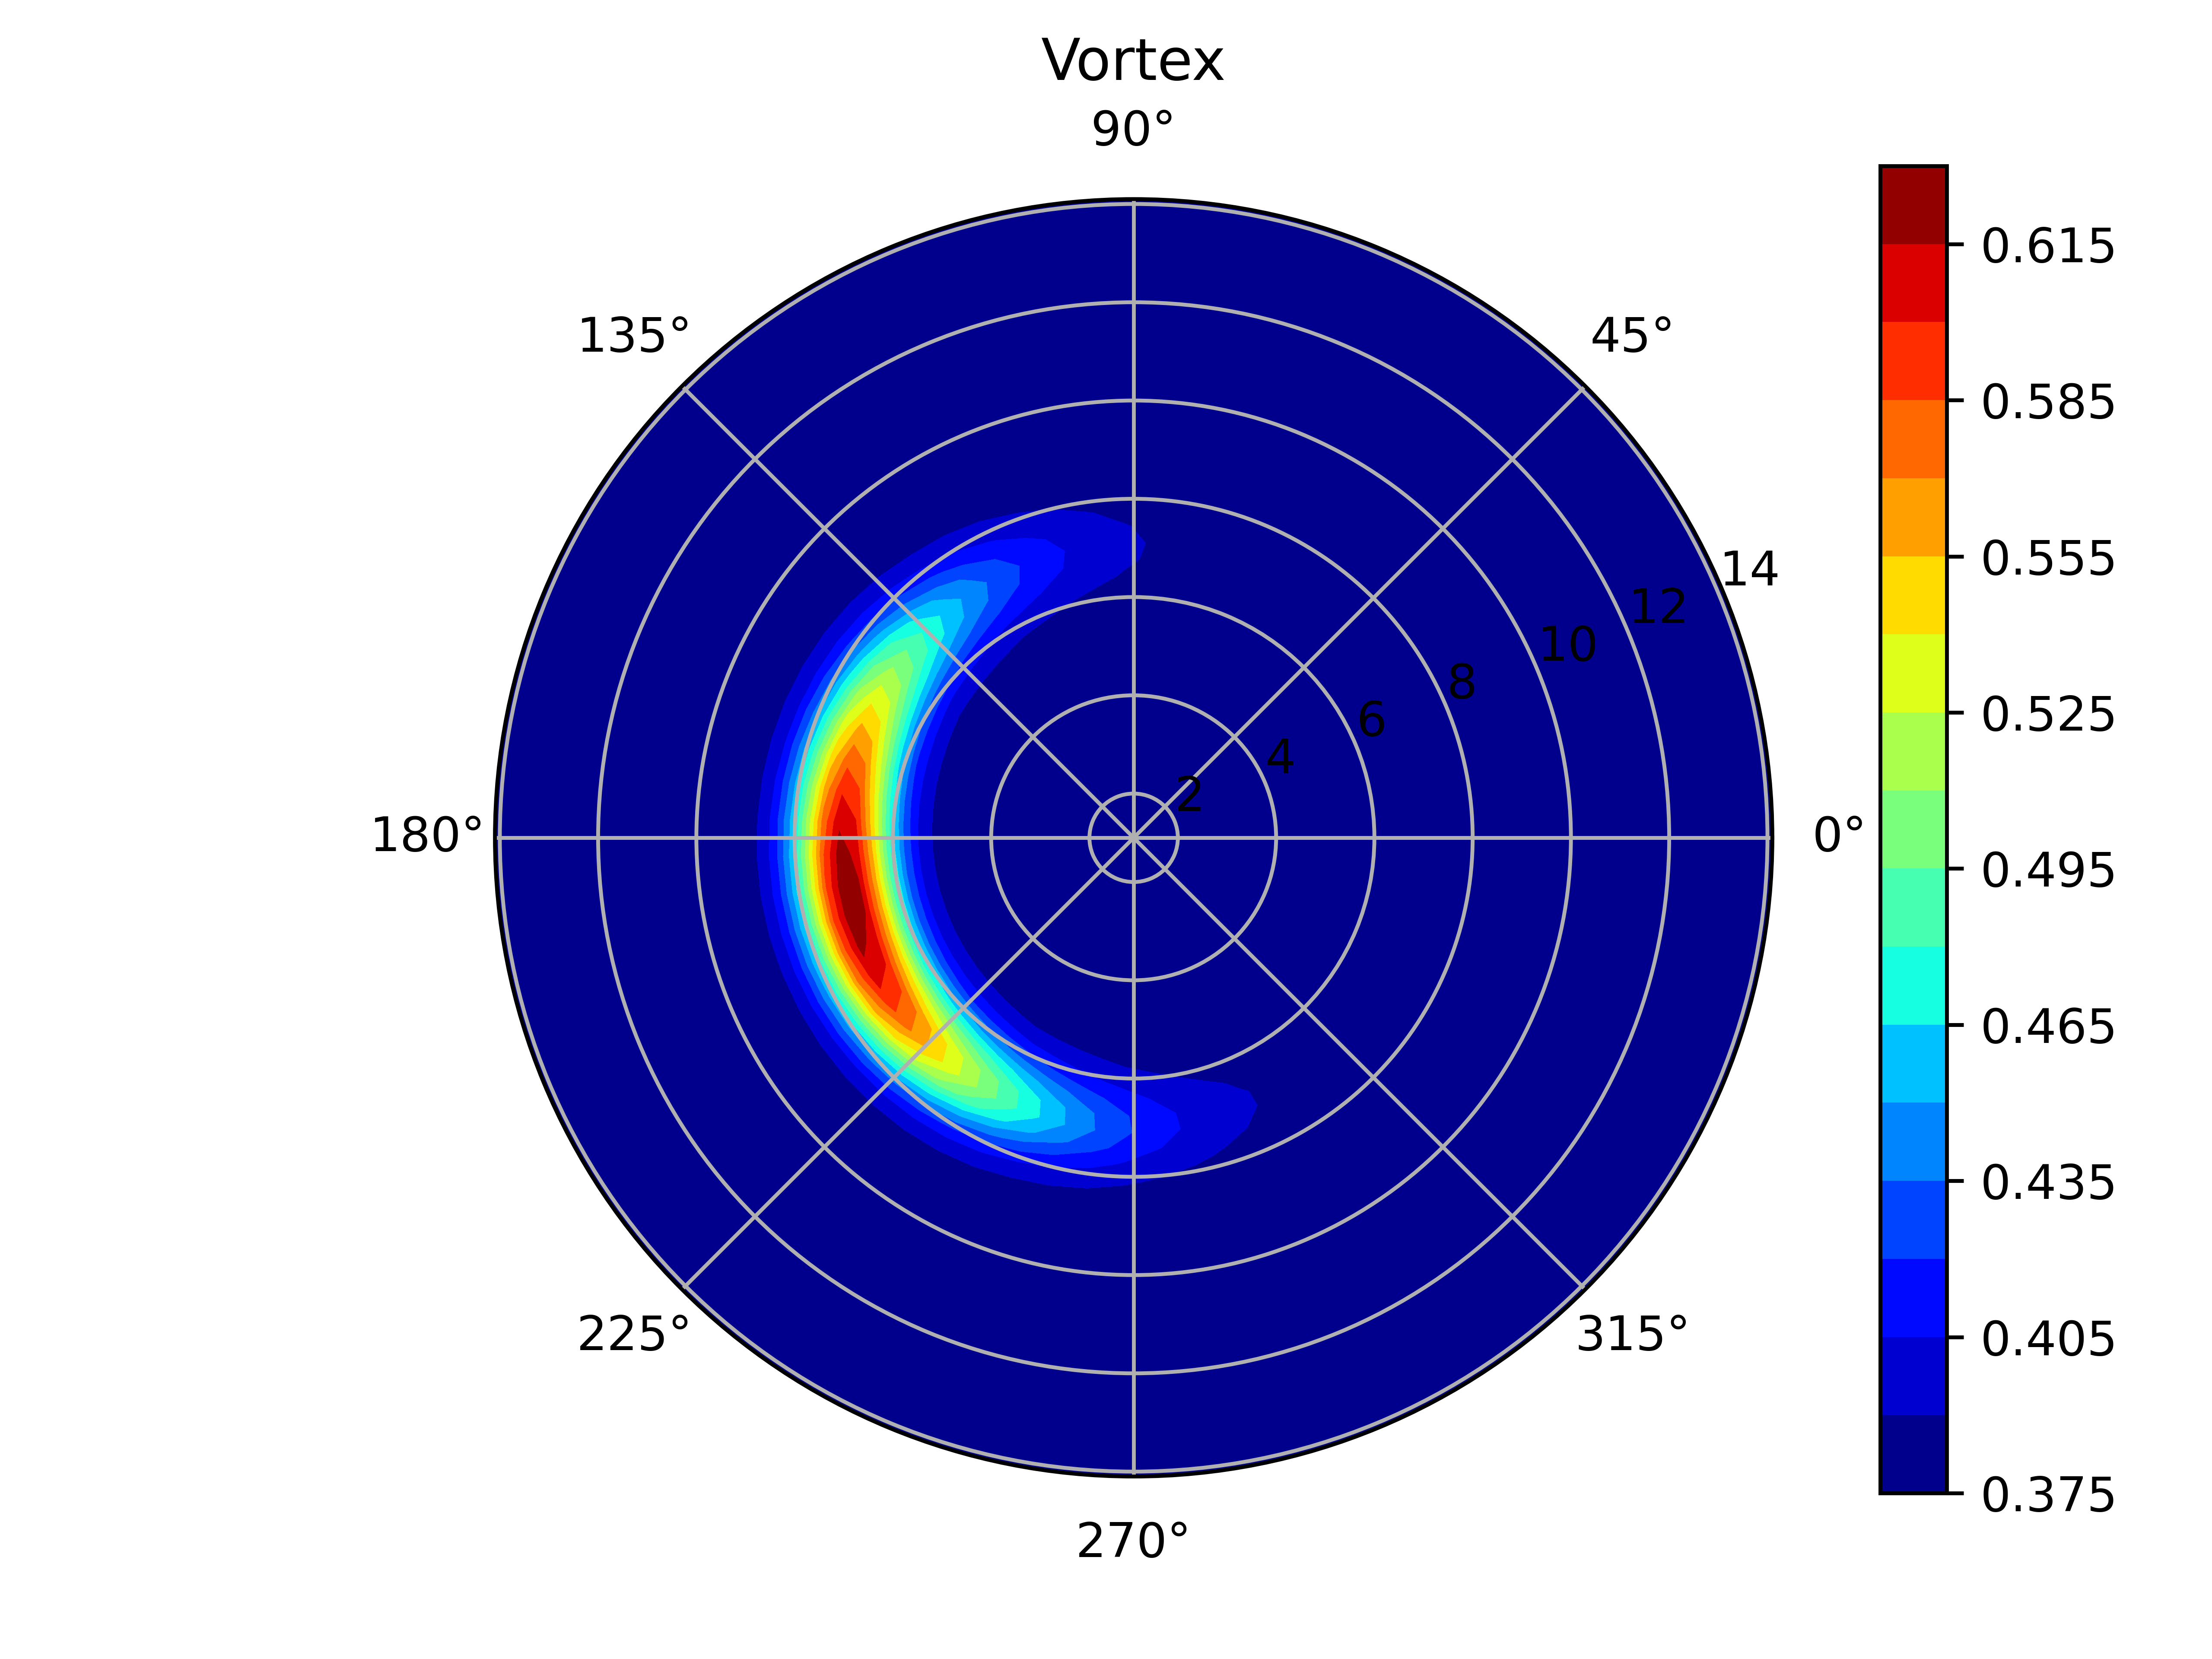
\includegraphics[width=0.45\linewidth]{plots/vortex_init.png}
	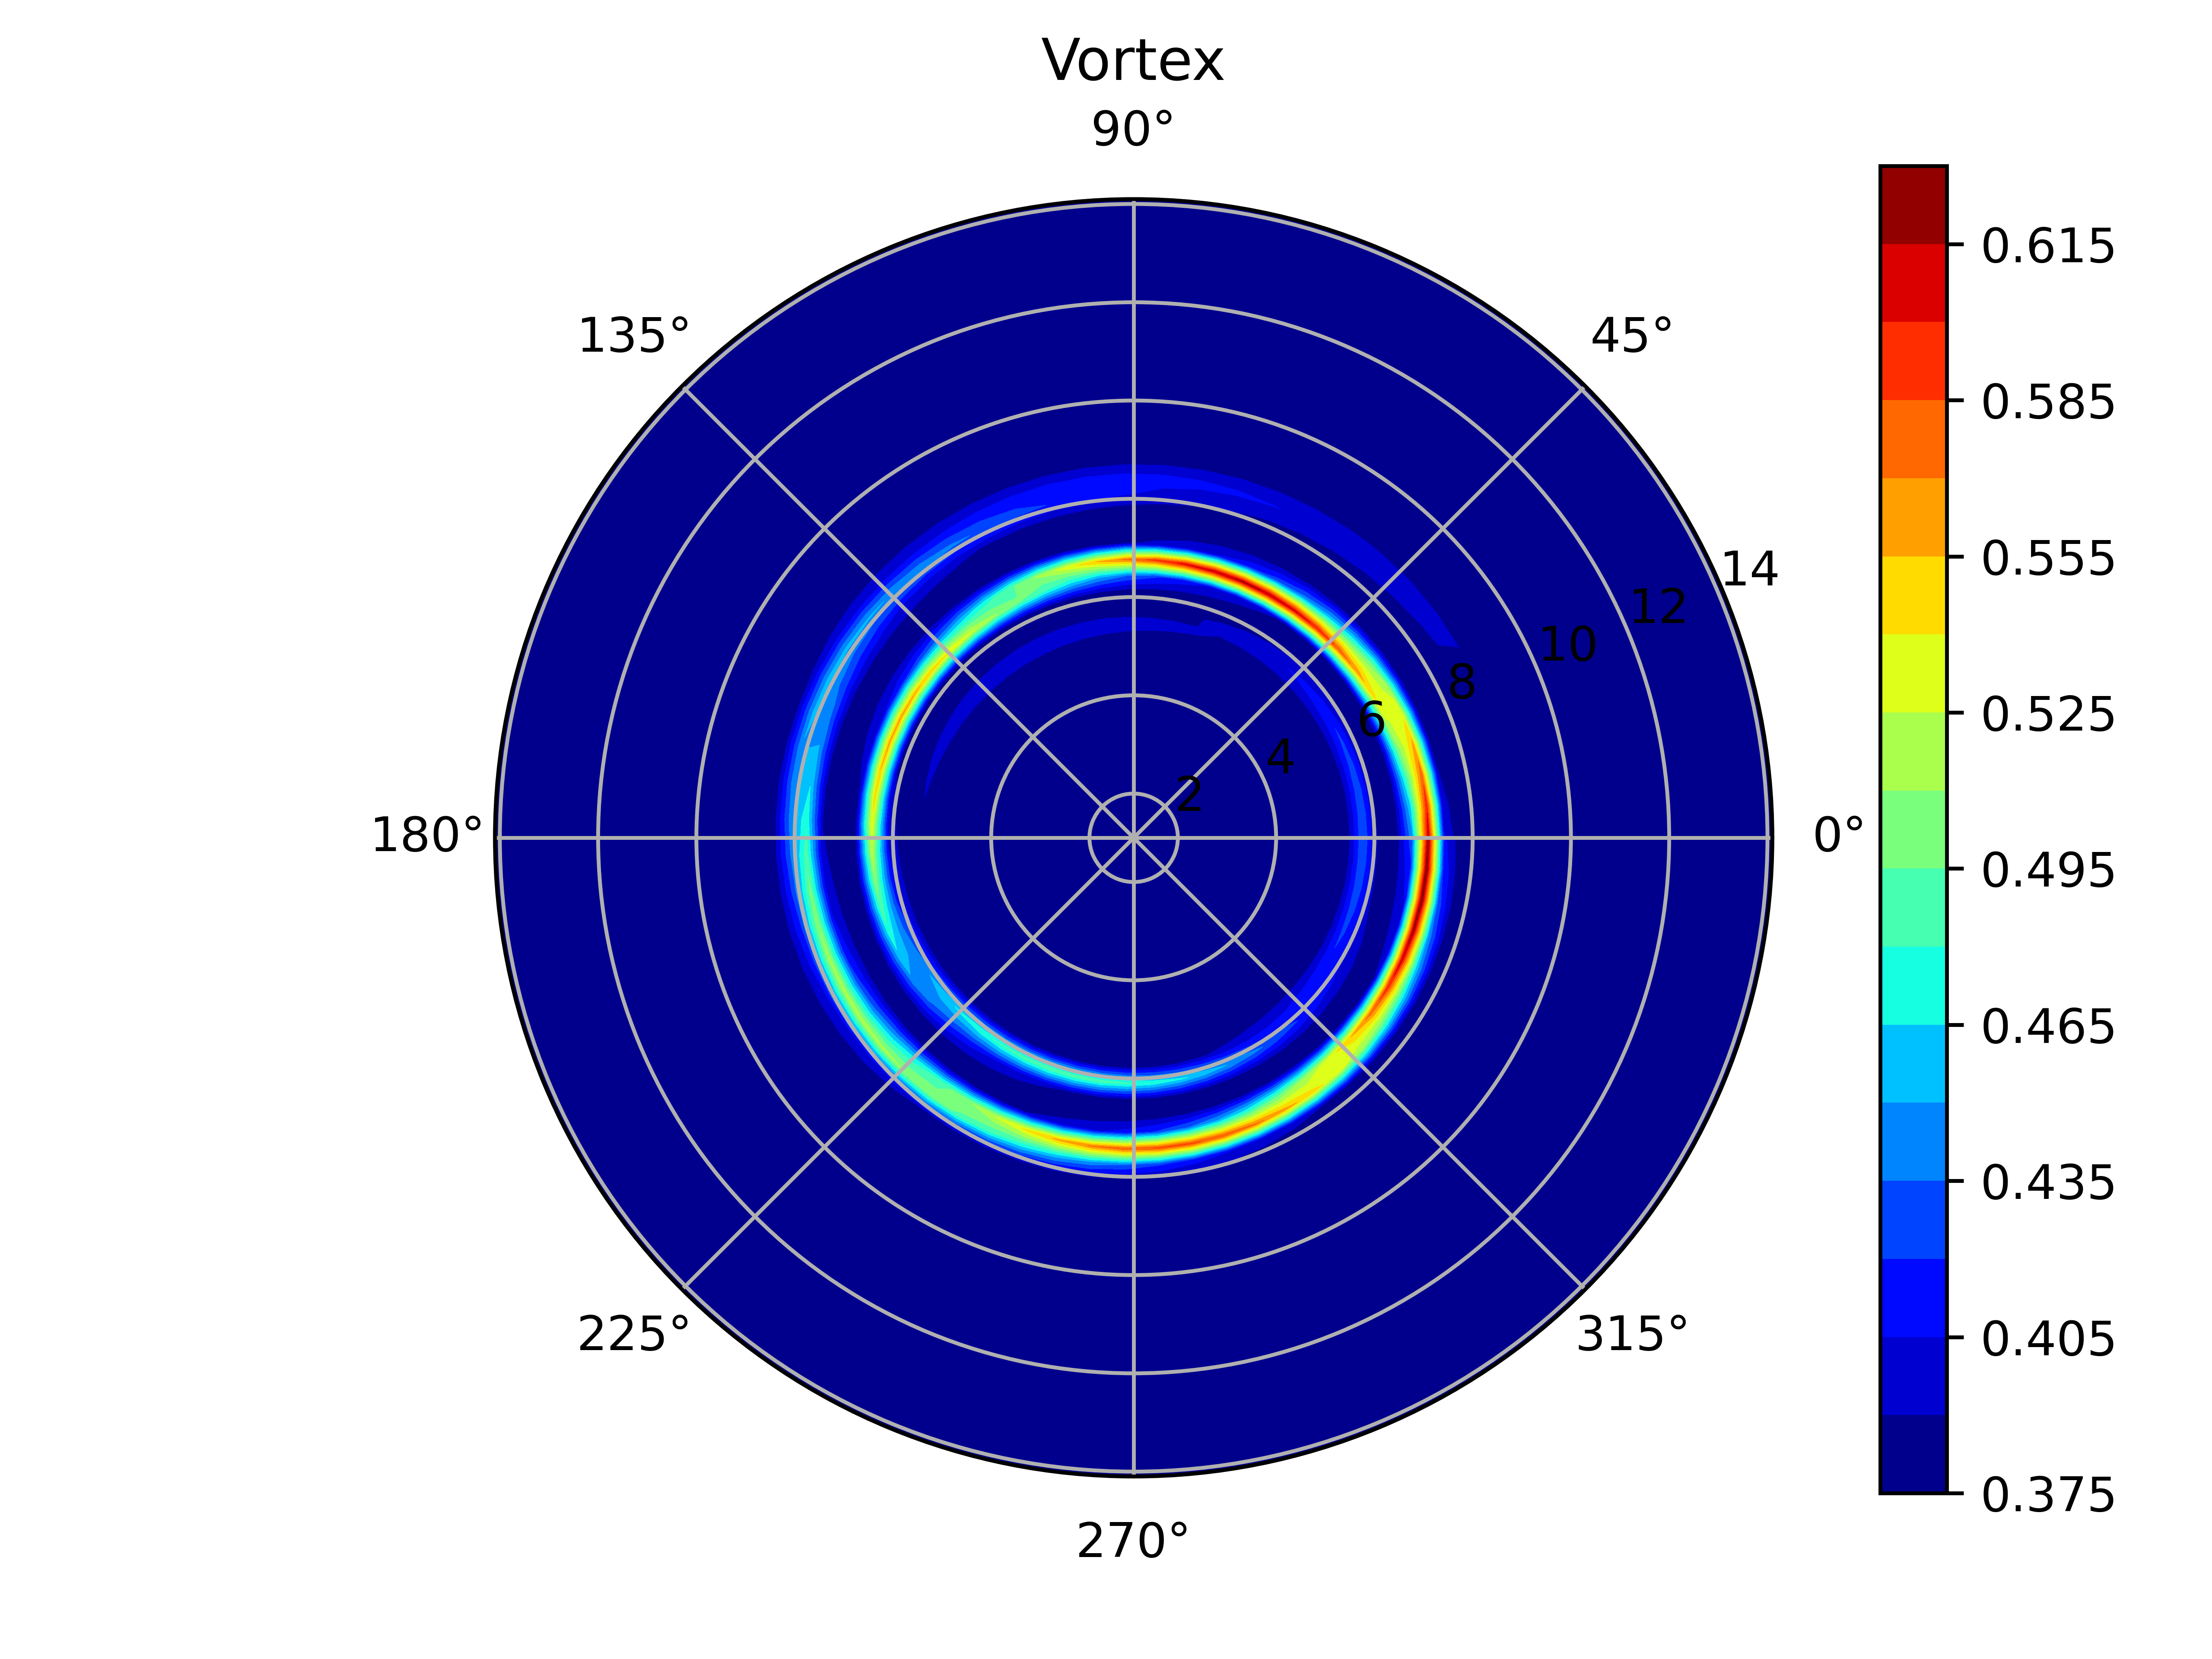
\includegraphics[width=0.45\linewidth]{plots/vortex_final.png}
	\caption{The density $f$ at initial (left) and final (right) time.}
	\label{fig:vortex}
\end{figure}

In order to solve this test-problem, we use the Arakawa scheme of order $4$, with an extrapolation of the equilibrium function as a boundary condition, as a space discretization, for which we divide the angular domain in $N_\theta = 60$ and radial domain in $N_r = 40$ cells. The time integration is done by an explicit Runge-Kutta scheme of order $4$, where we perform $N = 200$ time-steps with a step-size of $\Delta t = 0.1$.
\begin{figure}[h]
	\centering
	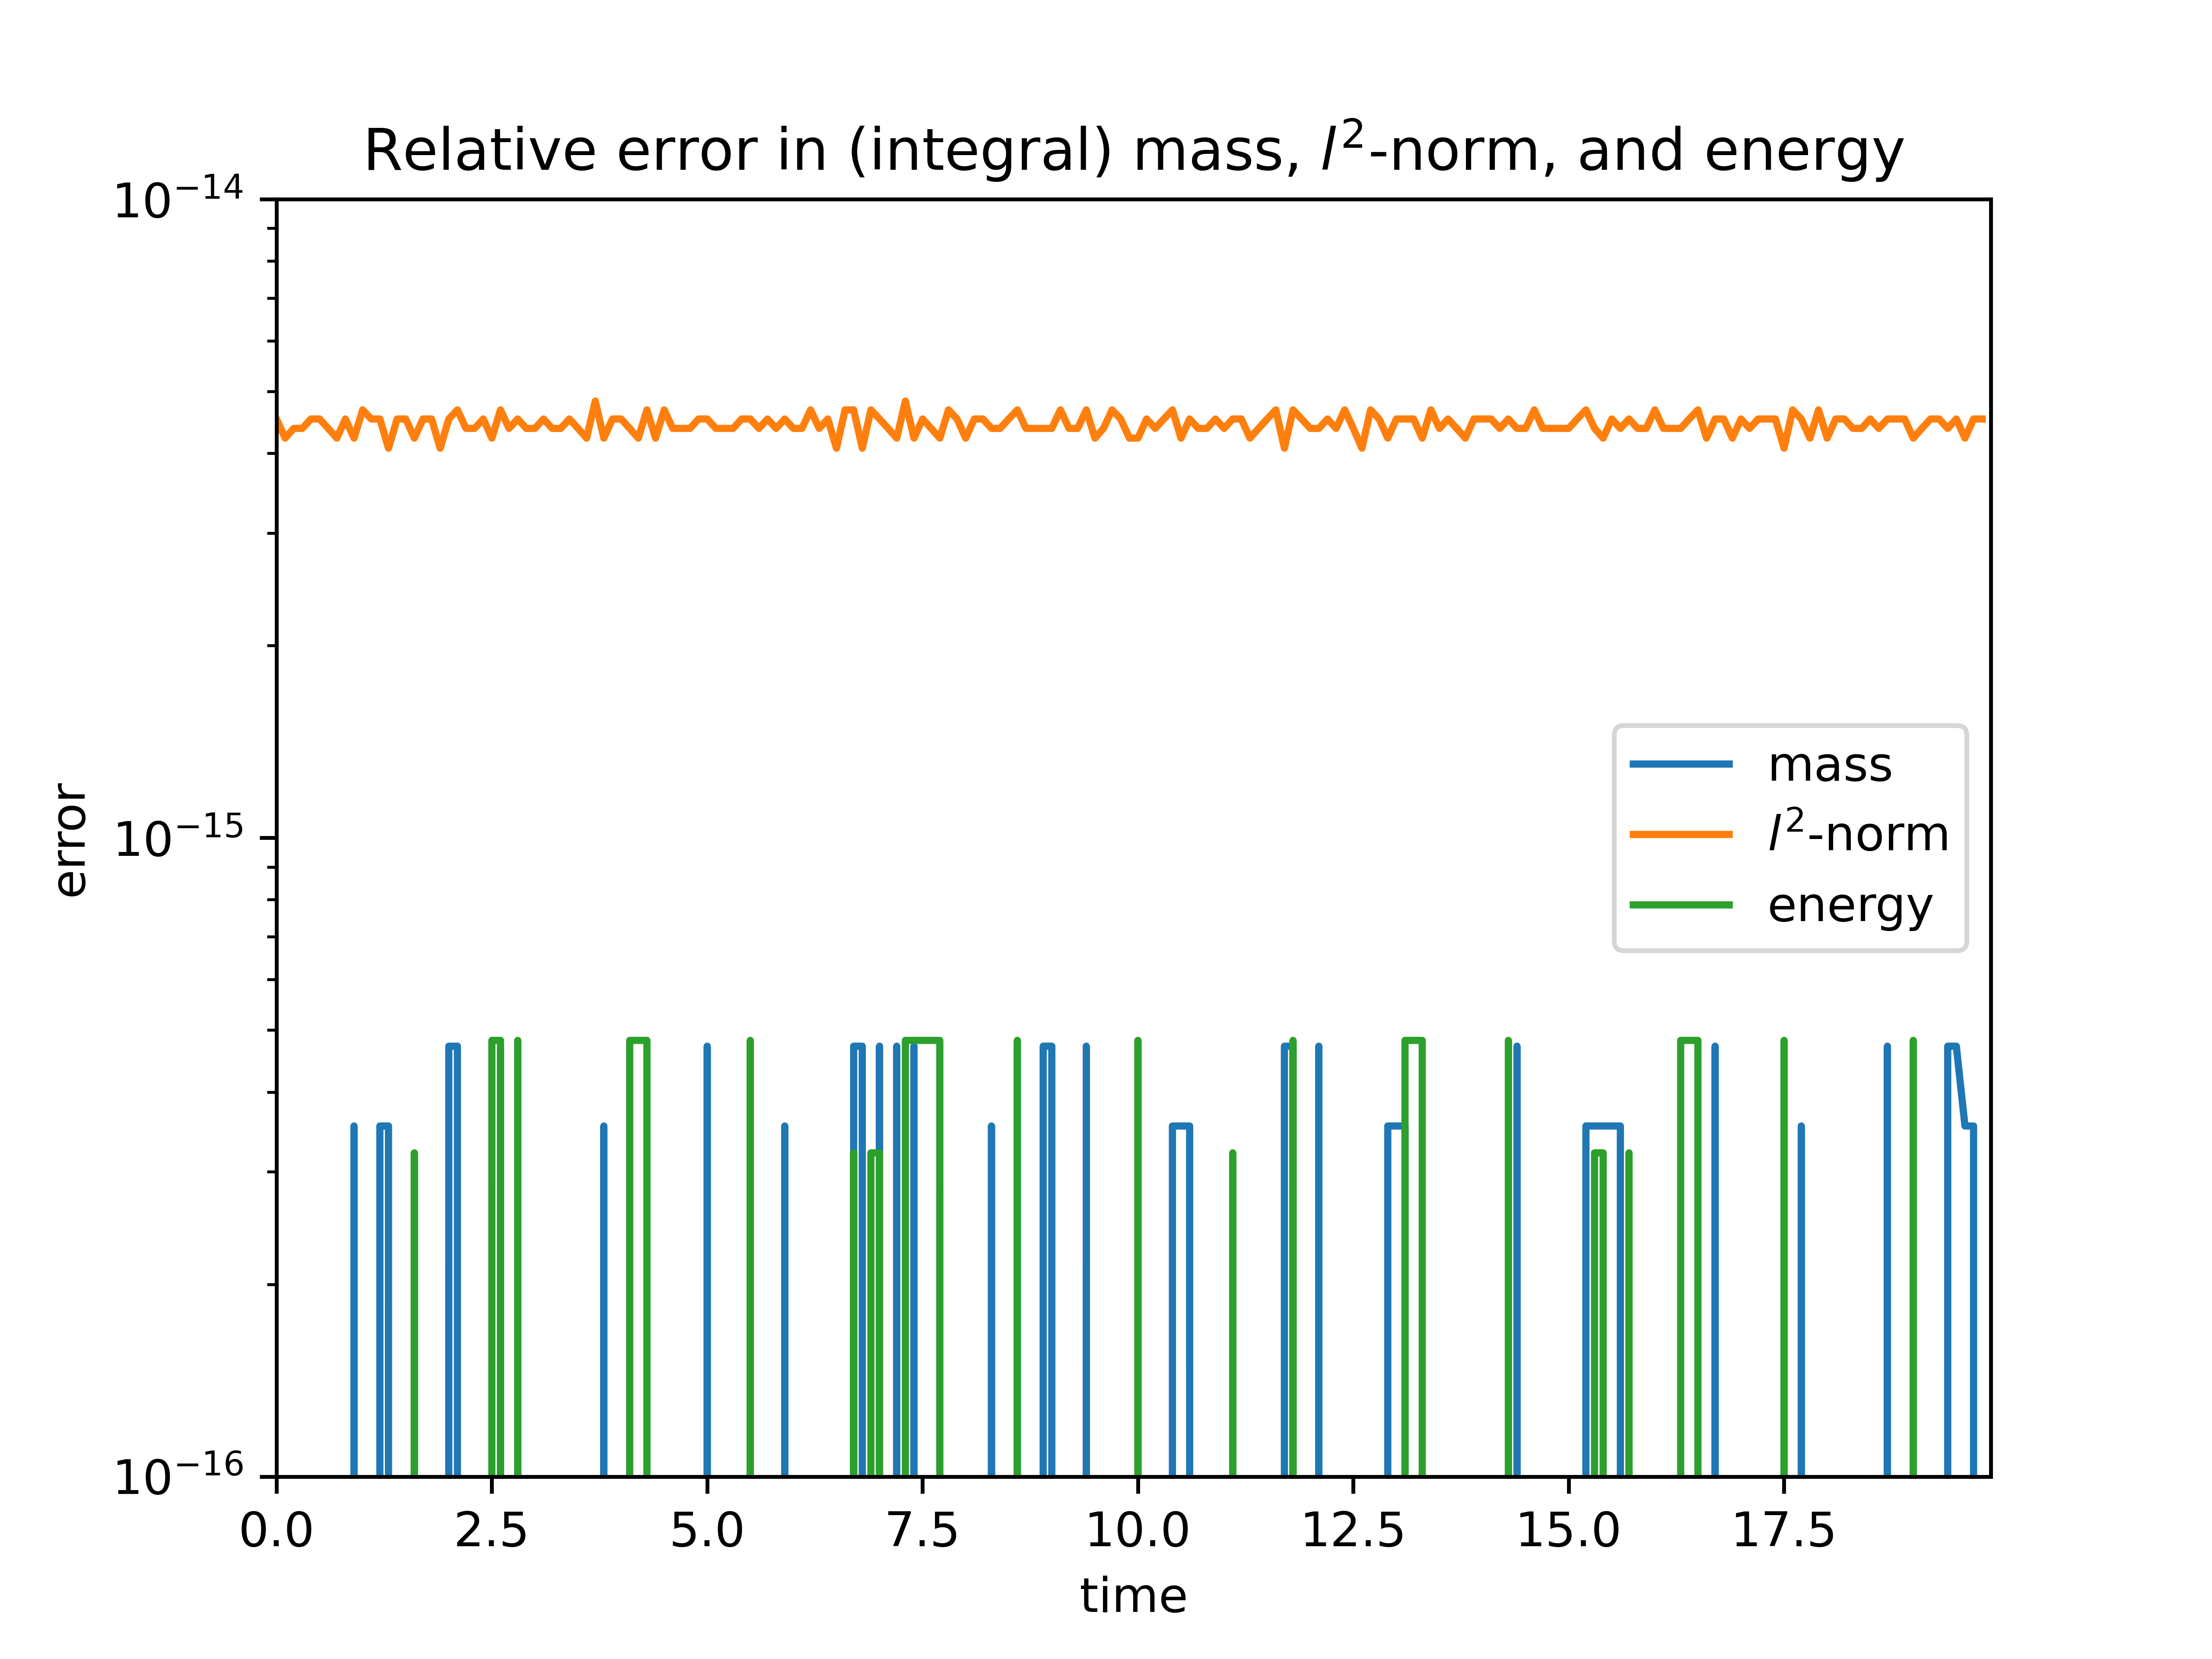
\includegraphics[width=0.45\linewidth]{plots/vortex_cons.png}
	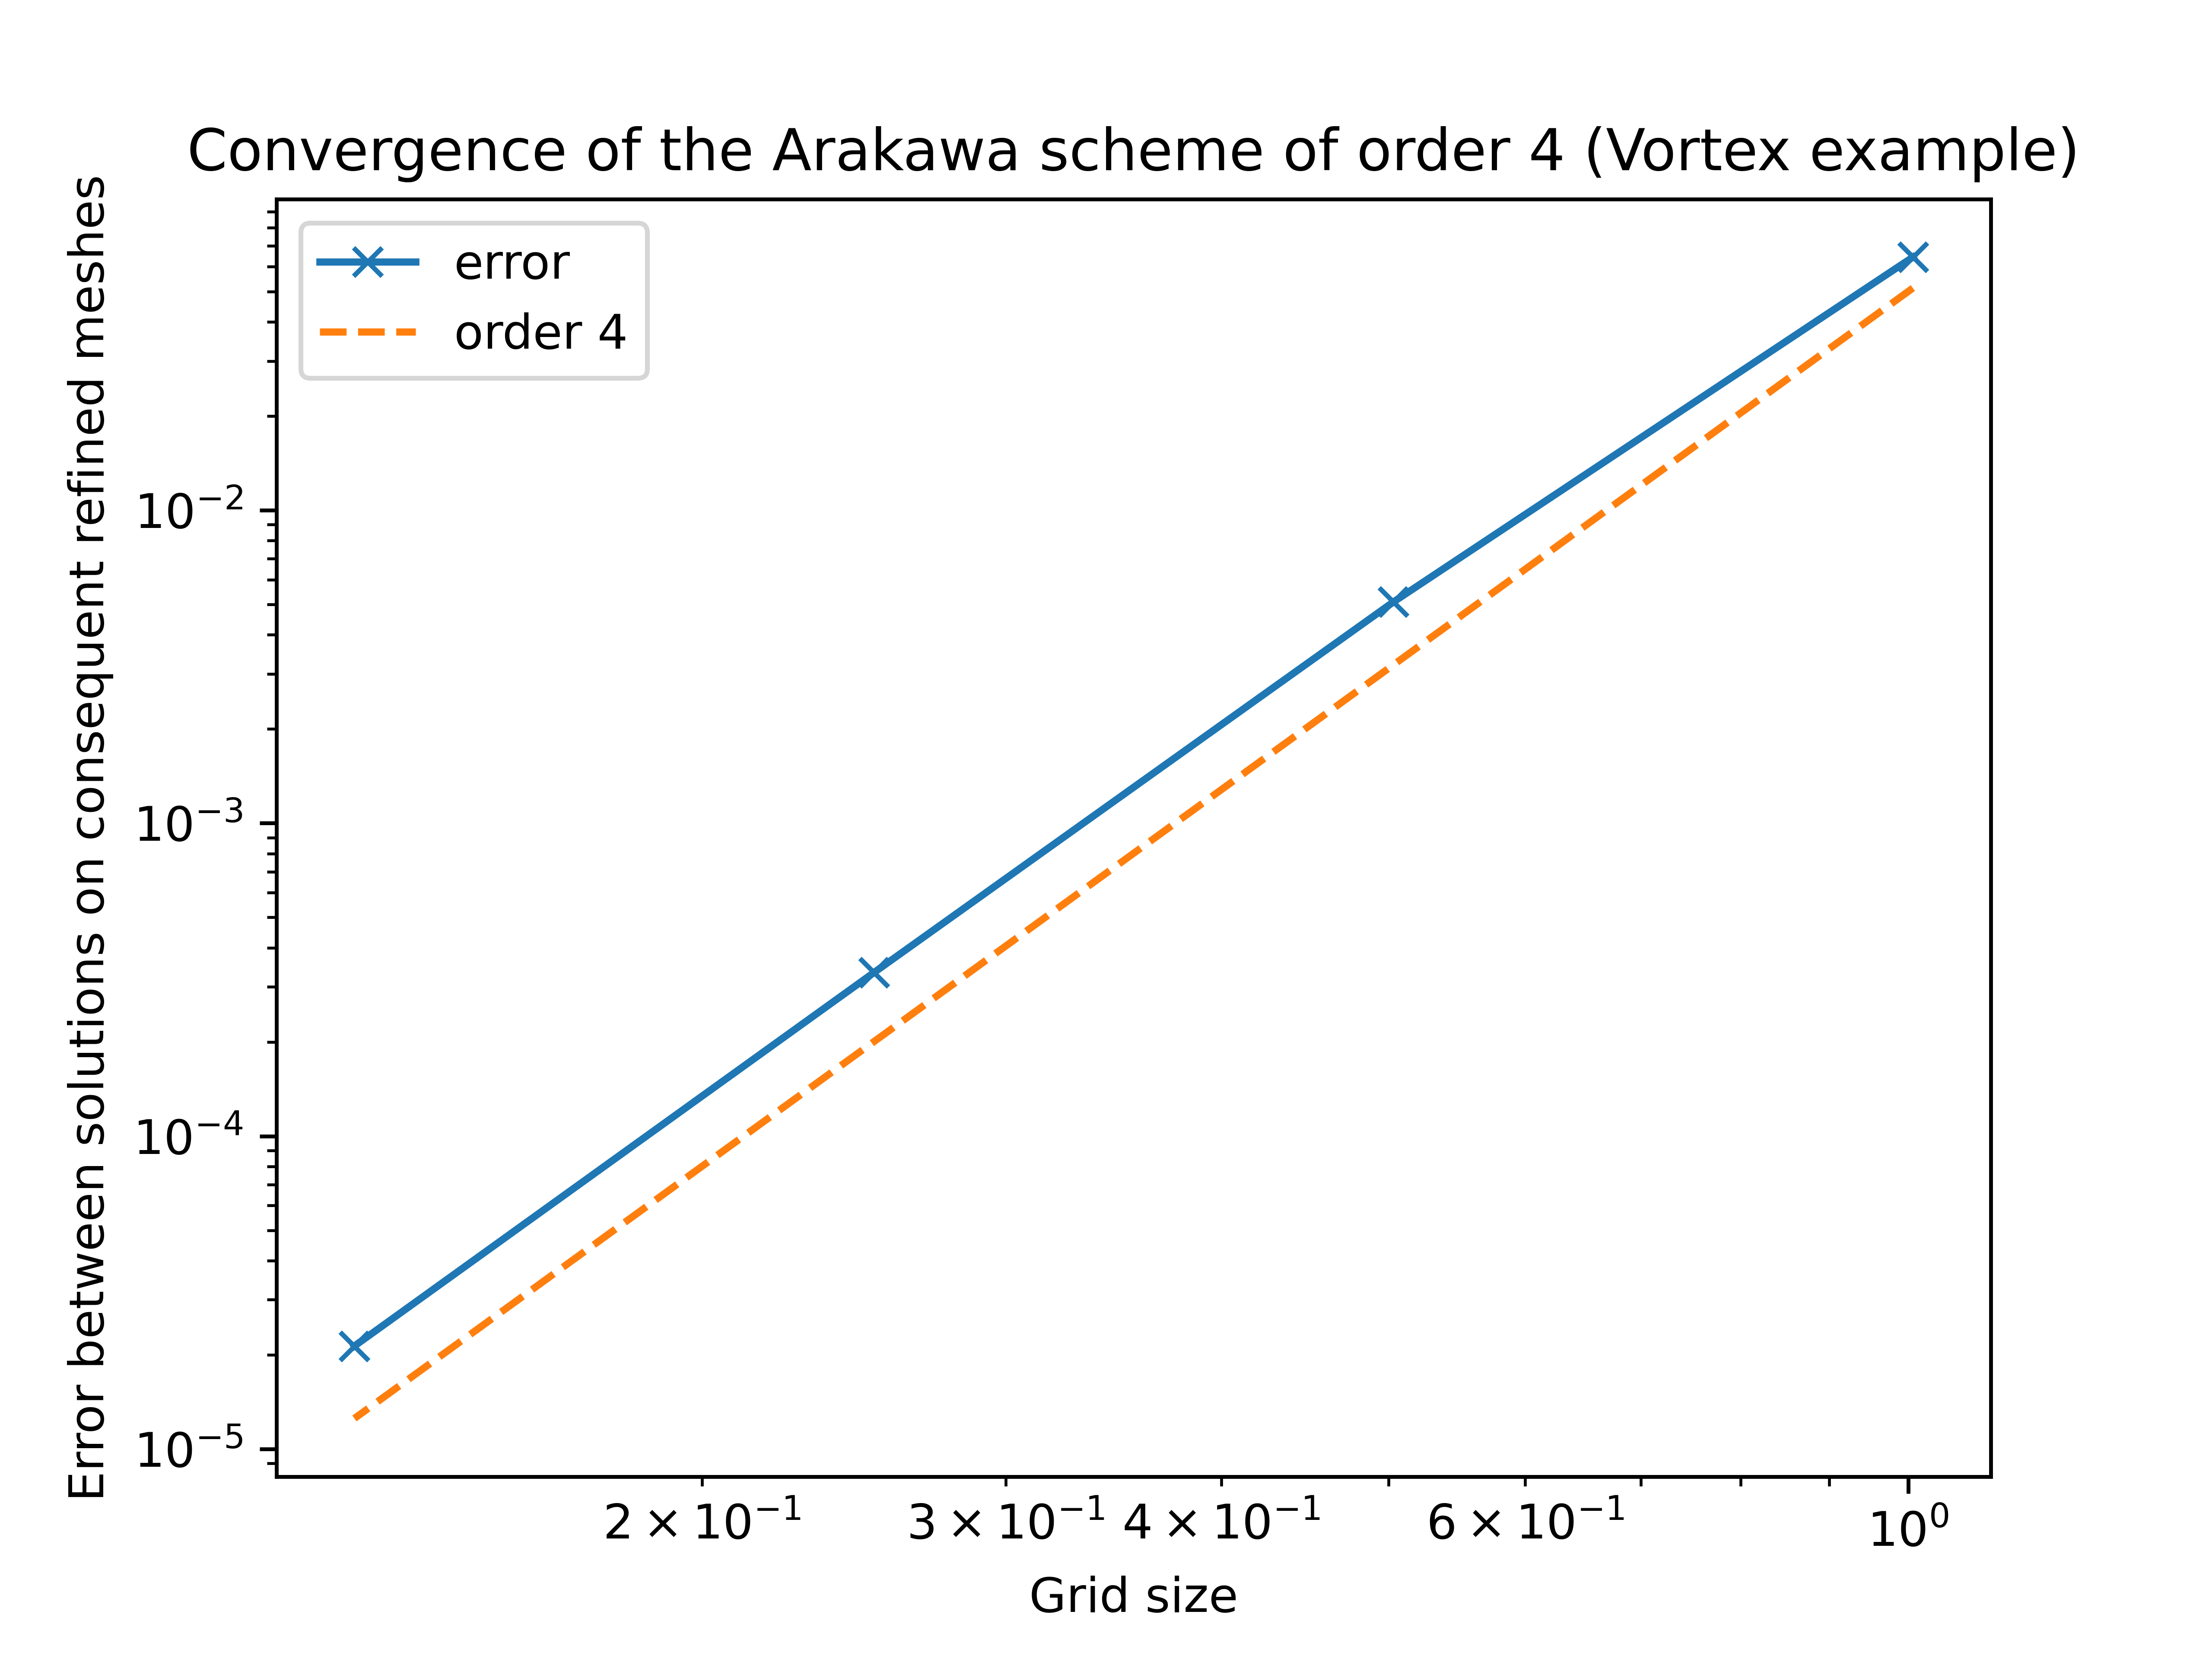
\includegraphics[width=0.45\linewidth]{plots/vortex_conv.png}
	\caption{Conservation of mass, $l^2$-norm and energy by the Arakawa scheme (left) and its order of convergence (right).}
	\label{fig:vortex_con}
\end{figure}
While solving, we keep track of the $l^1$-norm, or mass in other words, $l^2$-norm and the potential energy. As shown in \ref{fig:vortex_con}, these properties are preserved by the discrete solution as we have shown in section \ref{sec:consv-props}. Furthermore, we compare the relative error of our method on subsequently refined meshes in order to compute the order of convergence as shown in \ref{fig:vortex_con}.





\subsection{PyGyro}

Our main point of comparing the Arakawa method to the Semi-Lagrangian scheme are the conserved quantities: the mass
\begin{equation}
	\int f(r, \theta, z, v_\parallel) \d r \d \theta \d z \d v_\parallel
\end{equation}
and $l^2$-norm
\begin{equation}
	\left[\int f^2(r, \theta, z, v_\parallel) \d r \d \theta \d z \d v_\parallel\right]^\frac{1}{2}
\end{equation}
of the distribution function, and the potential energy
\begin{equation}
	\int \left(f(r, \theta, z, v_\parallel) - f_\text{eq}(r, v_\parallel)\right) \Phi(r, \theta, z) \d r \d \theta \d z \d v_\parallel
\end{equation}
, as well as the not necessarily conserved kinetic energy
\begin{equation}
	\int \left(f(r, \theta, z, v_\parallel) - f_\text{eq}(r, v_\parallel)\right) v^2_\parallel \d r \d \theta \d z \d v_\parallel
\end{equation}

From a simulation with grid size $[r:128, \theta:256, z:128, v_\parallel :72]$ and time step-size $\Delta t = 1$ we plot for the above mentioned 4 quantities the absolute error (figure \ref{fig:abserr}), the relative error (figure \ref{fig:relerr}), and the relative error on a logarithmic scale (\ref{fig:relerrlog}) before and after the poloidal advection step.

We can clearly see that the Arakawa scheme preserves the conserved quantities much better than semi-Lagrangian scheme. In the linear phase, the error is of order of machine precision. Only very late in the non-linear phase becomes the relative error bigger, but is still one or two orders of magnitude smaller than in the semi-Lagrangian scheme.

The kinetic energy is also much better preserved.

The same study with time-step size $\Delta t = 2$ was done (figures \ref{fig:abserr_dt2}, \ref{fig:relerr_dt2}, \ref{fig:relerrlog_dt2}) and yields the same results. It is therefore interesting to compare the results of the poloidal advection step for the Arakawa method for the two time step-sizes; these results are shown in figures \ref{fig:abserr_akw}, \ref{fig:relerr_akw}, \ref{fig:relerrlog_akw}. We see that the doubling of the time step-size results in double the absolute error for the conserved quantities, and about a factor of 5 for the kinetic energy.

%TODO: Only log scale probably
\begin{figure}
	\centering
	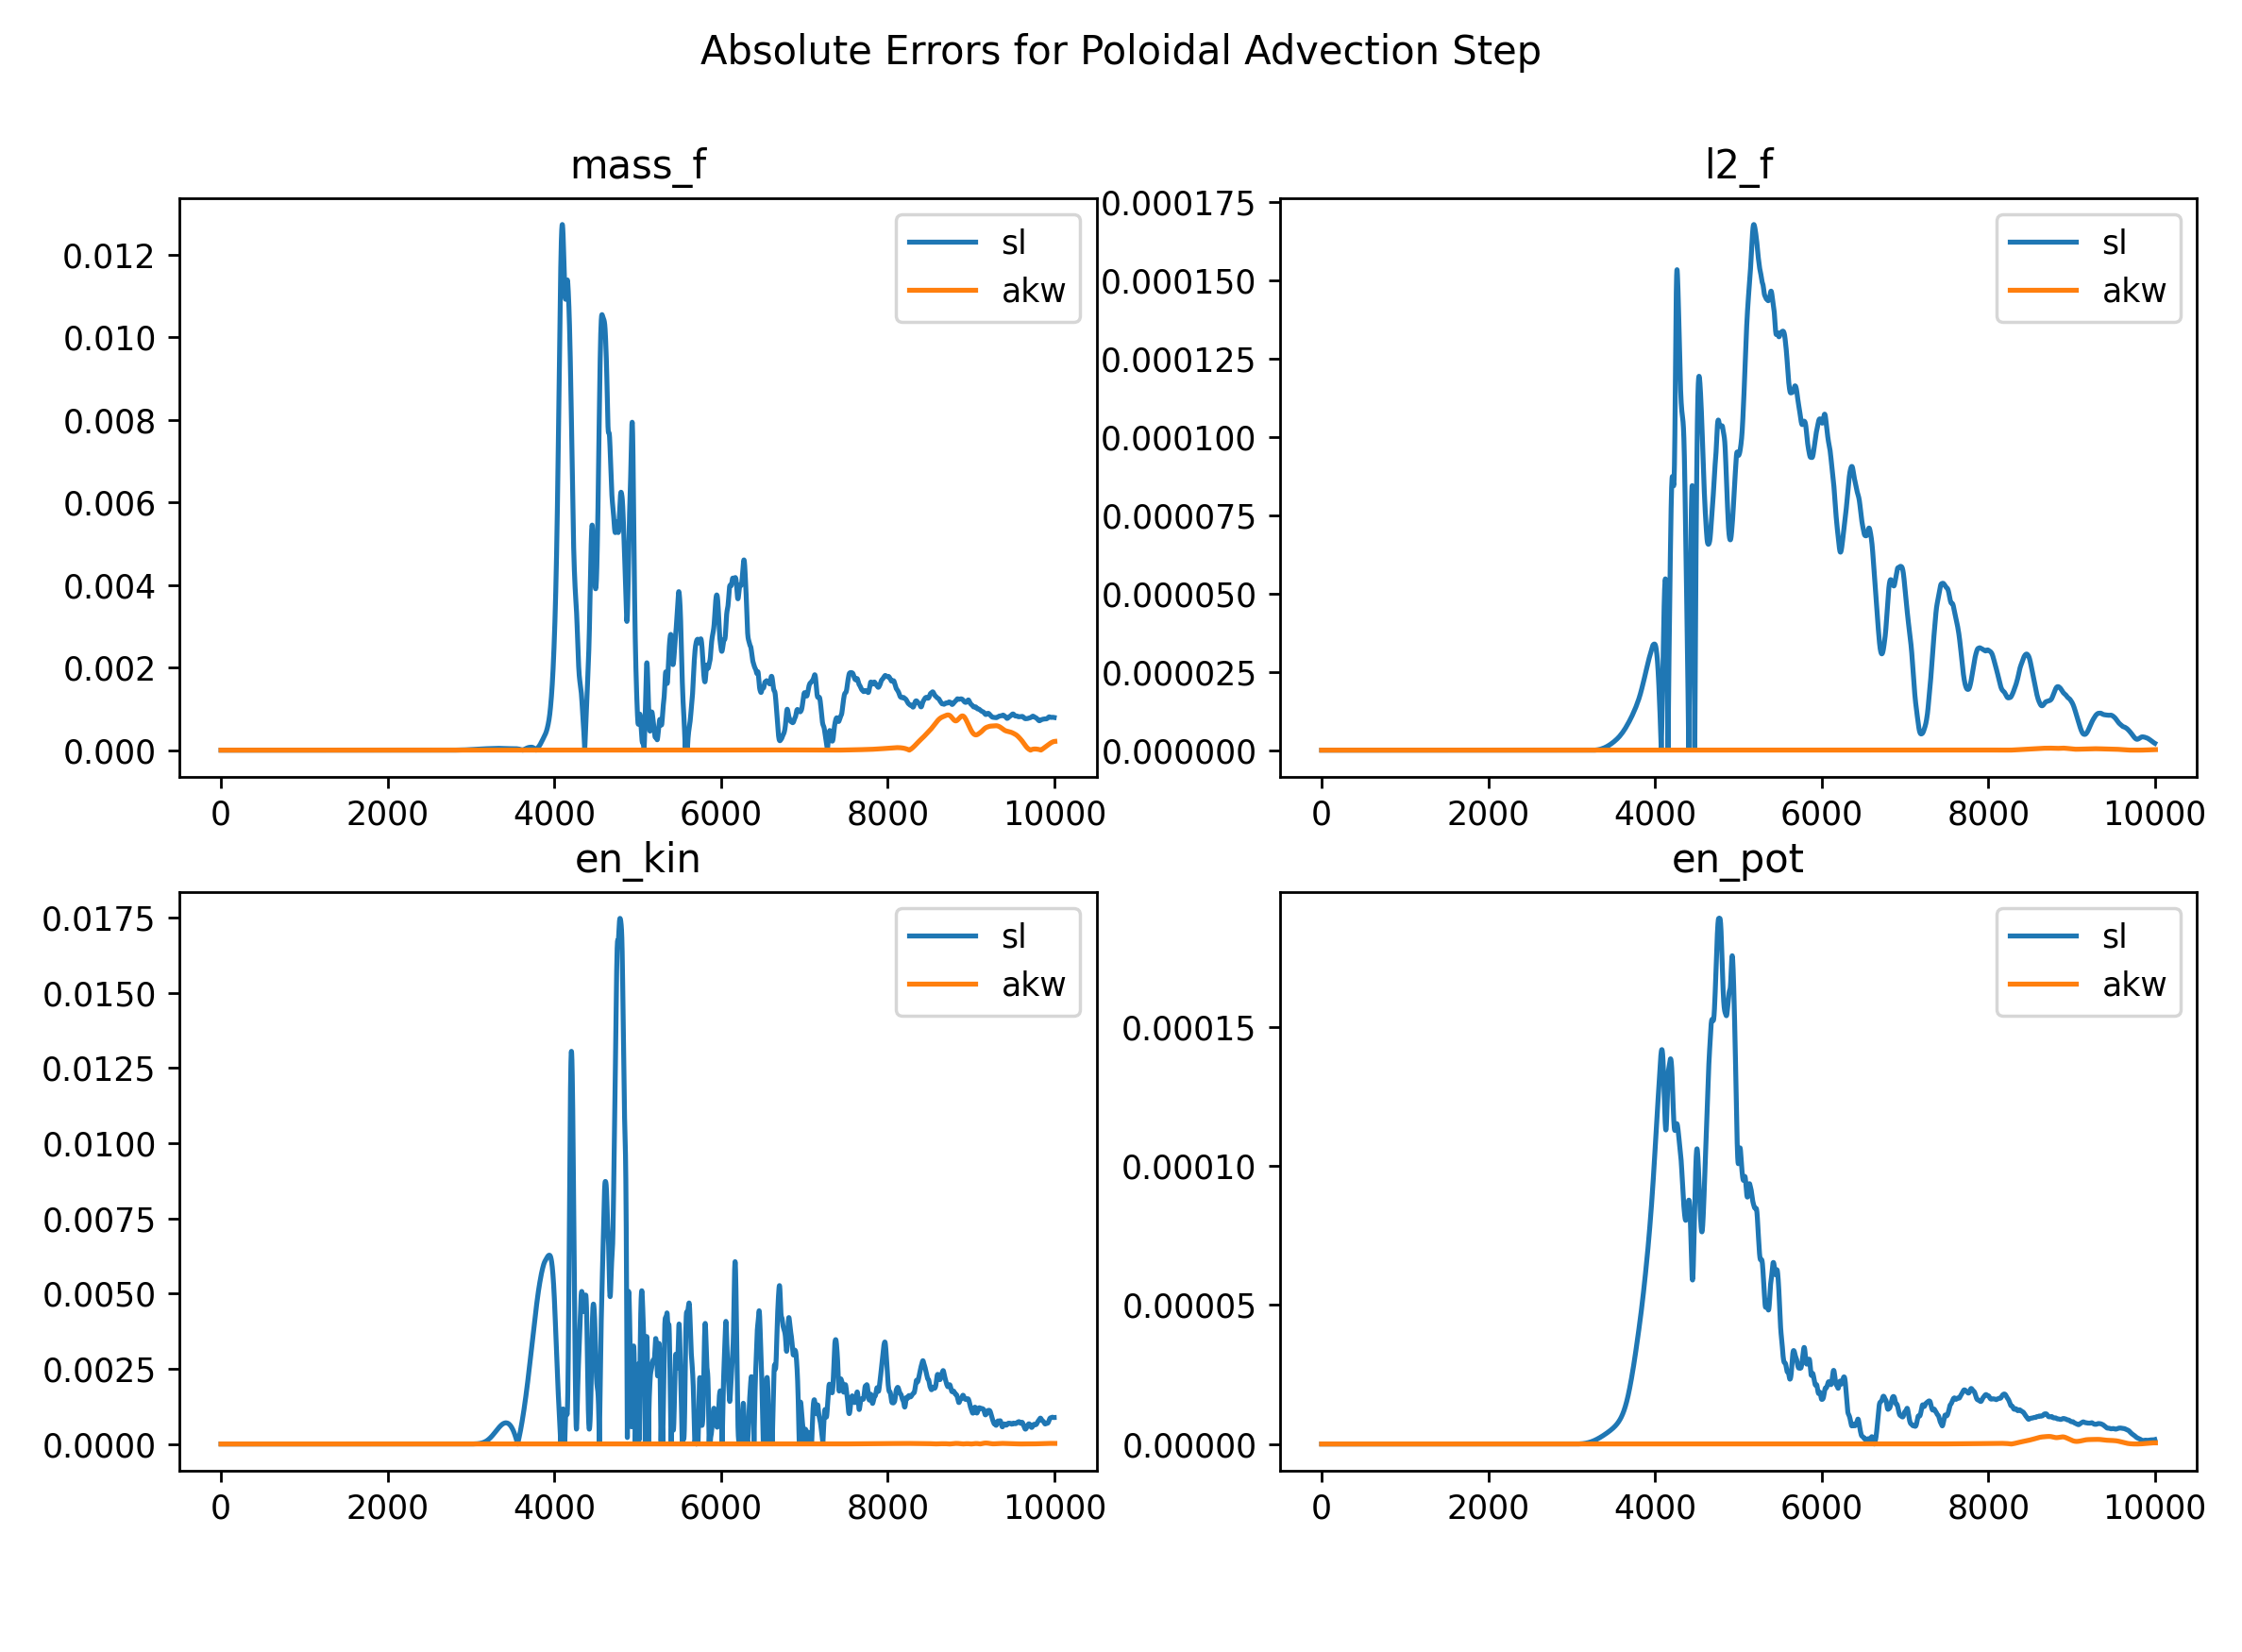
\includegraphics[width=0.9\linewidth]{plots/abs_err}
	\caption{The absolute error for different quantities before and after the poloidal advection step.}
	\label{fig:abserr}
\end{figure}


\begin{figure}
	\centering
	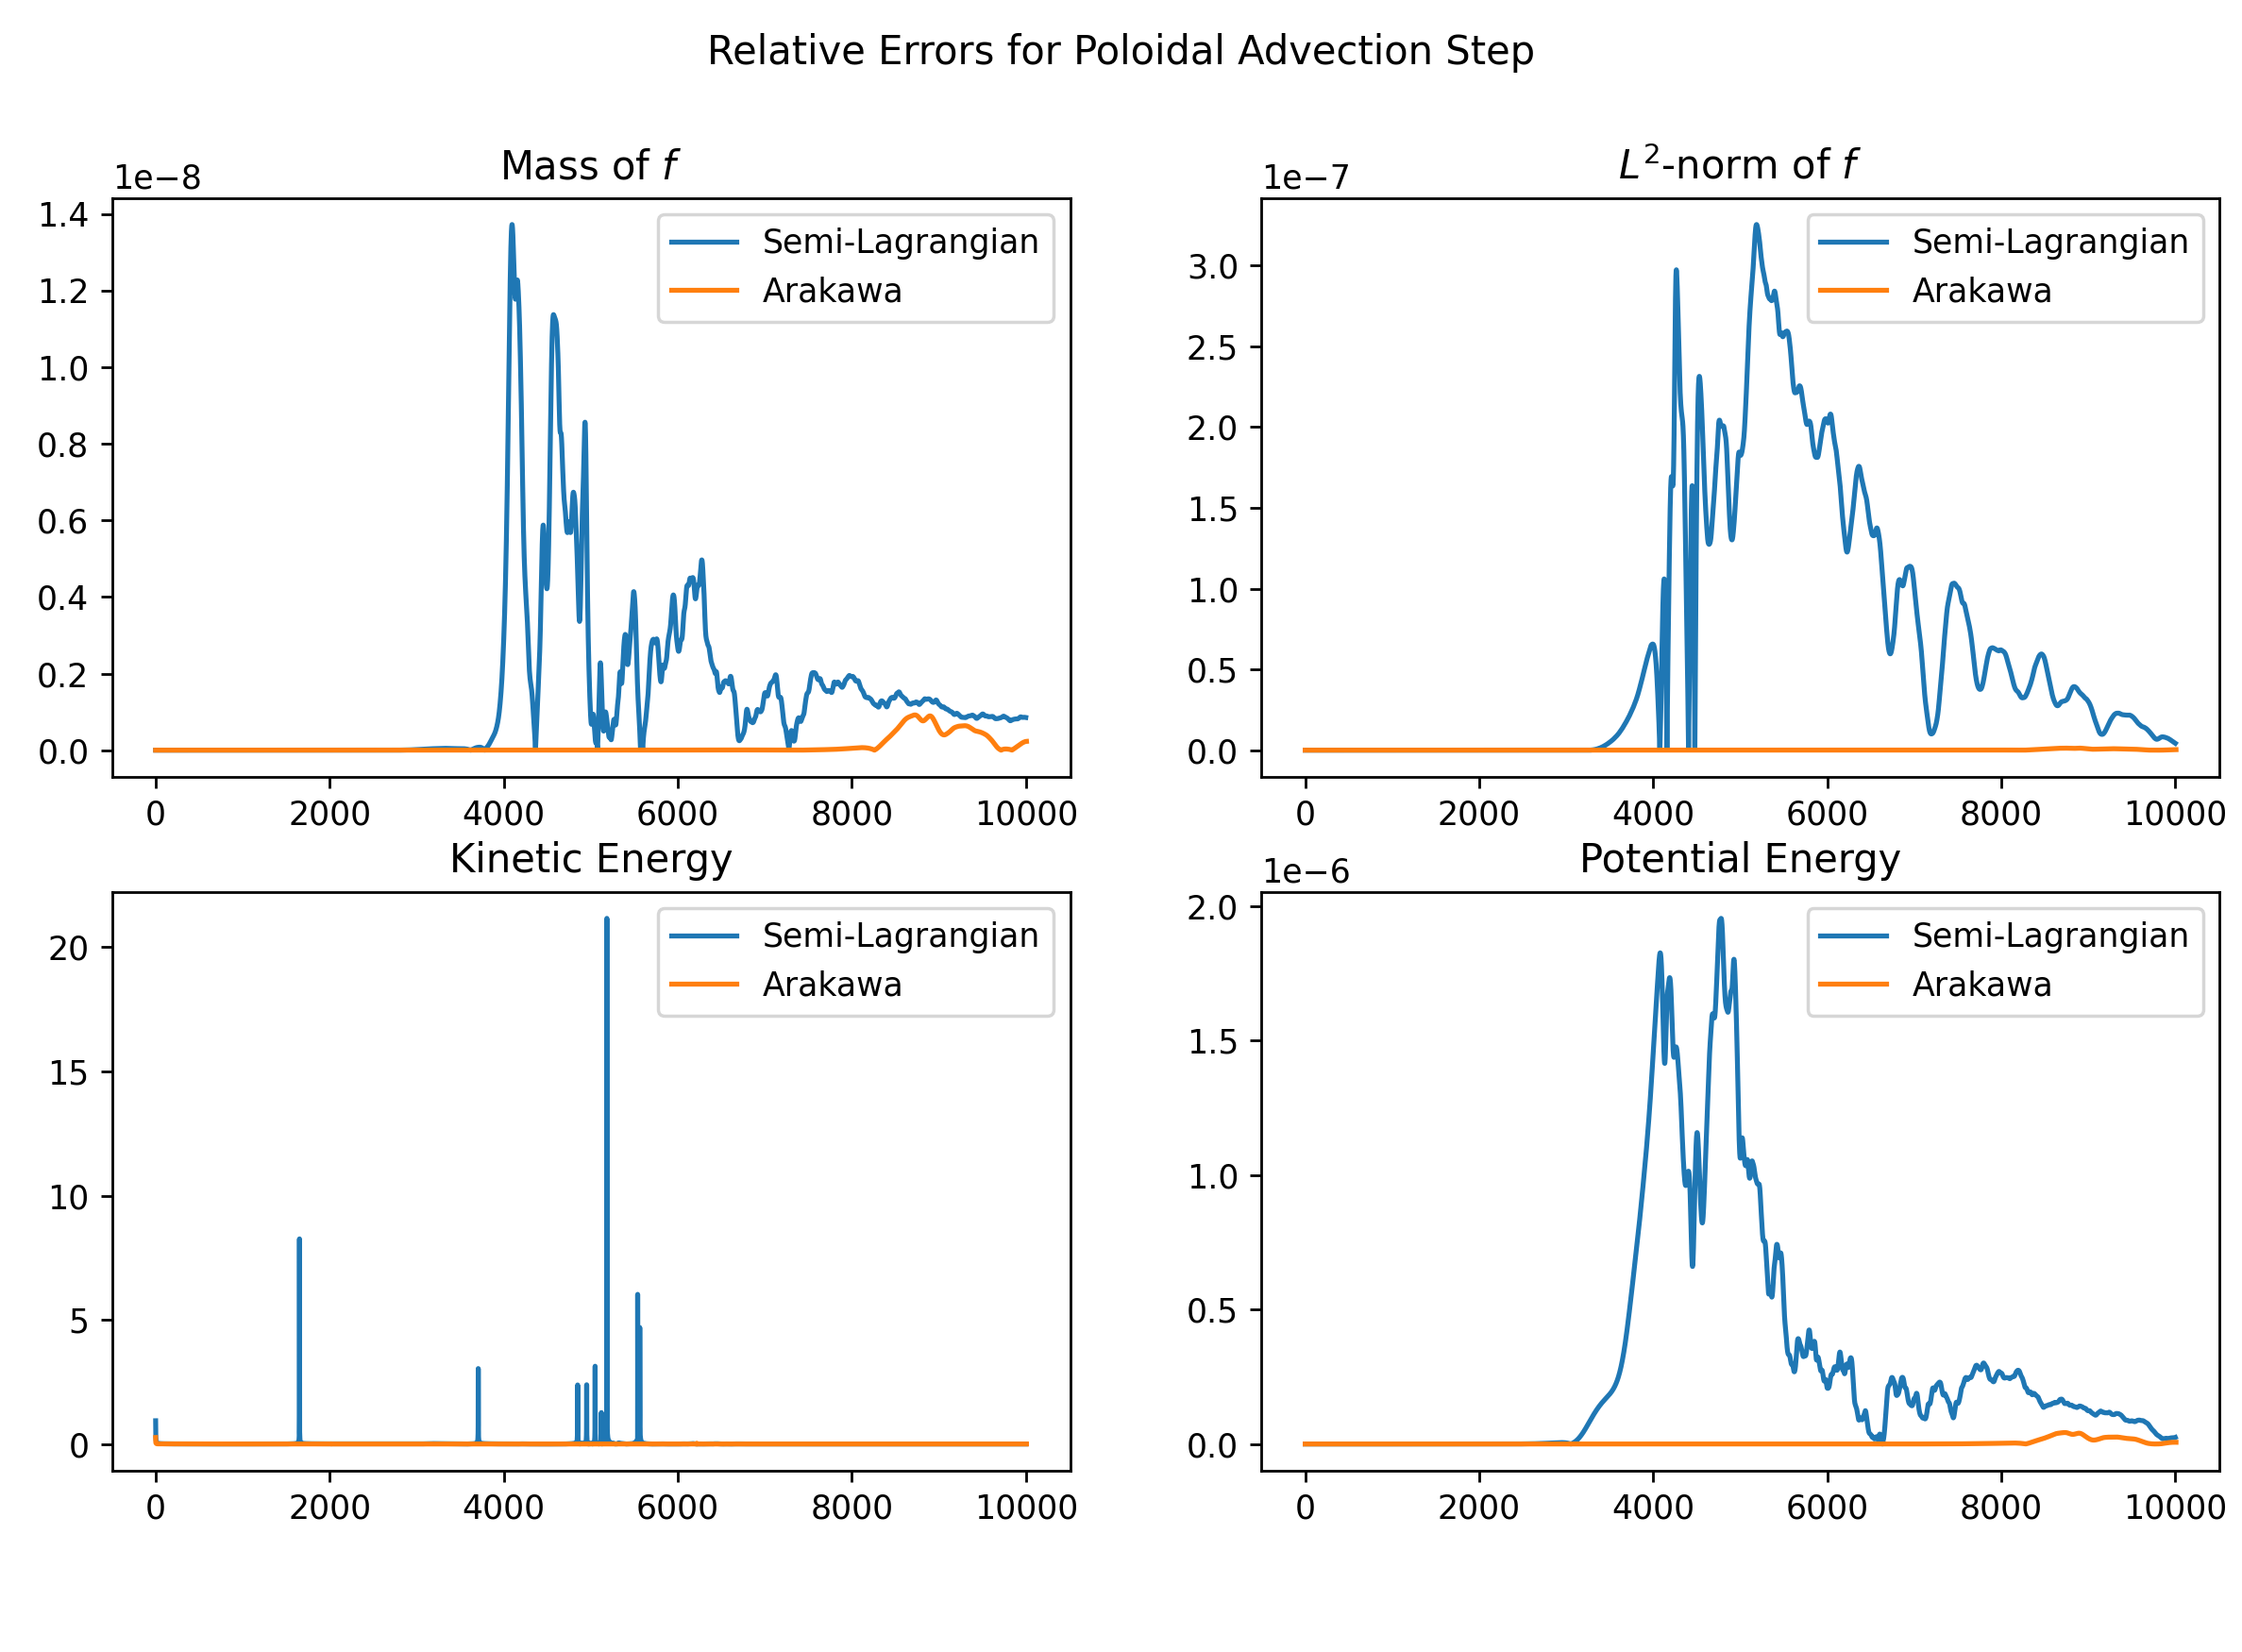
\includegraphics[width=0.9\linewidth]{plots/rel_err}
	\caption{The relative error for different quantities before and after the poloidal advection step.}
	\label{fig:relerr}
\end{figure}


\begin{figure}
	\centering
	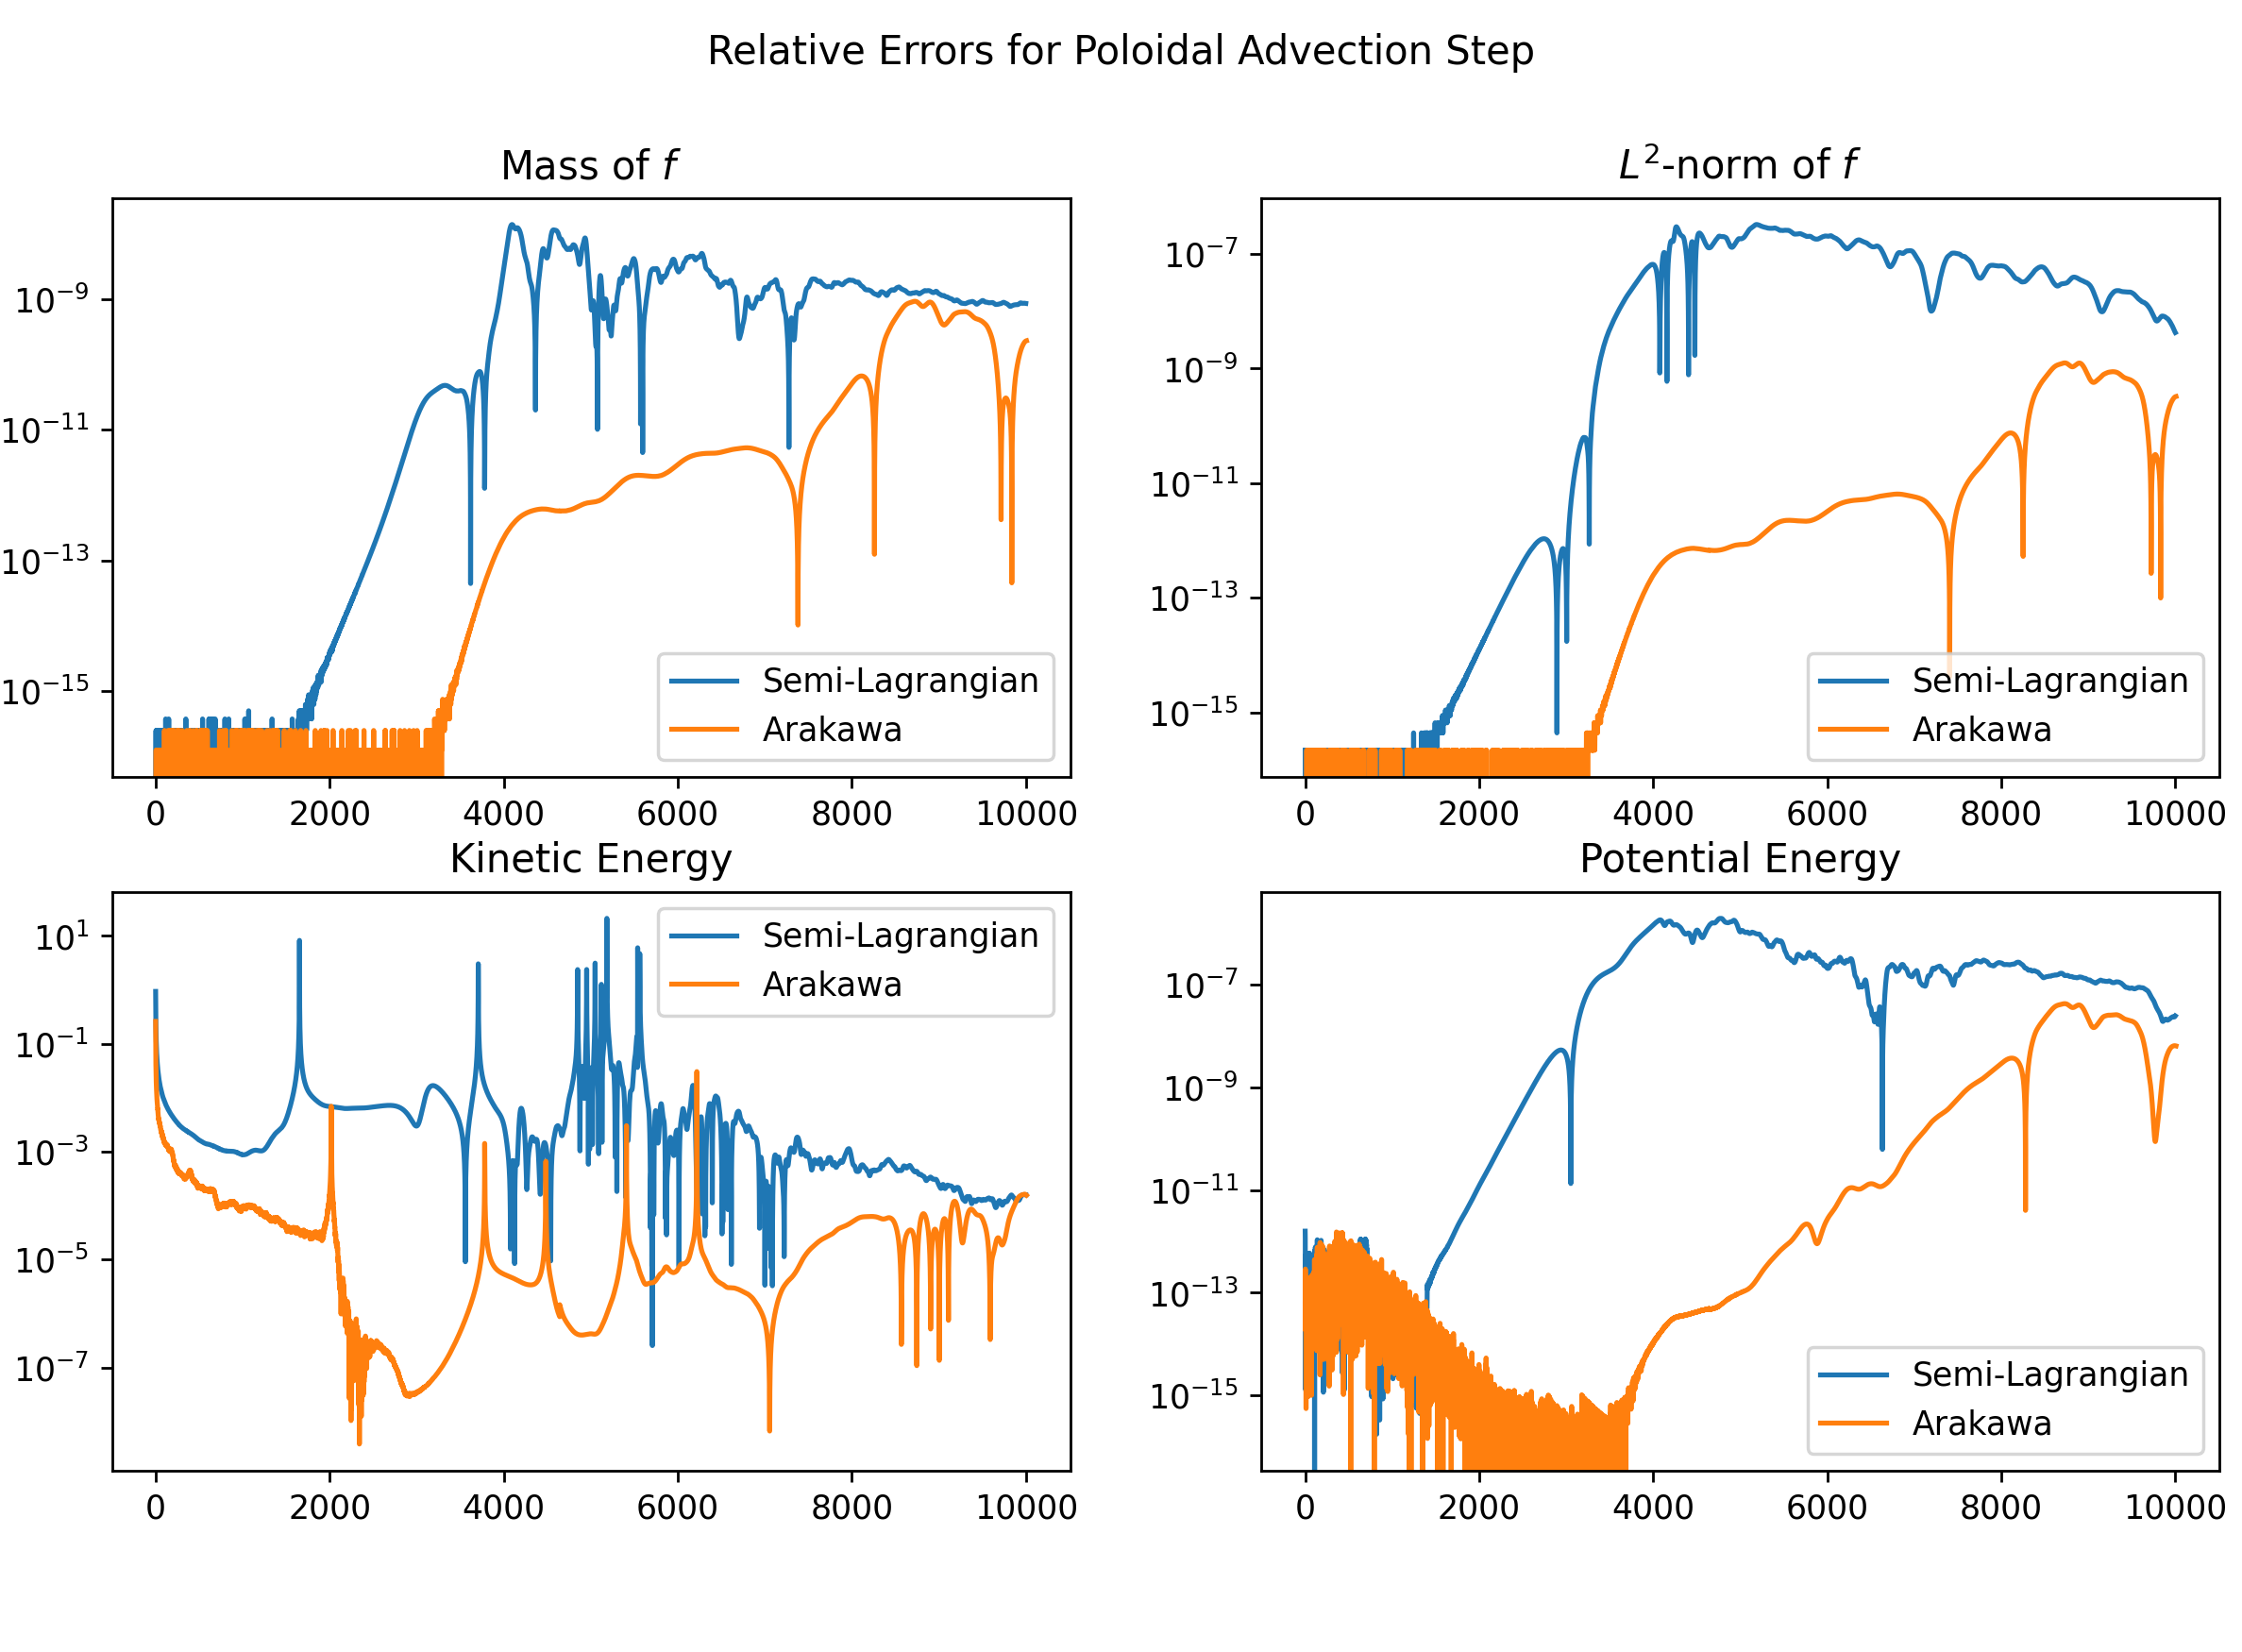
\includegraphics[width=0.9\linewidth]{plots/rel_err_log}
	\caption{The relative error for different quantities before and after the poloidal advection step on a semi-logarithmic scale.}
	\label{fig:relerrlog}
\end{figure}


\begin{figure}
	\centering
	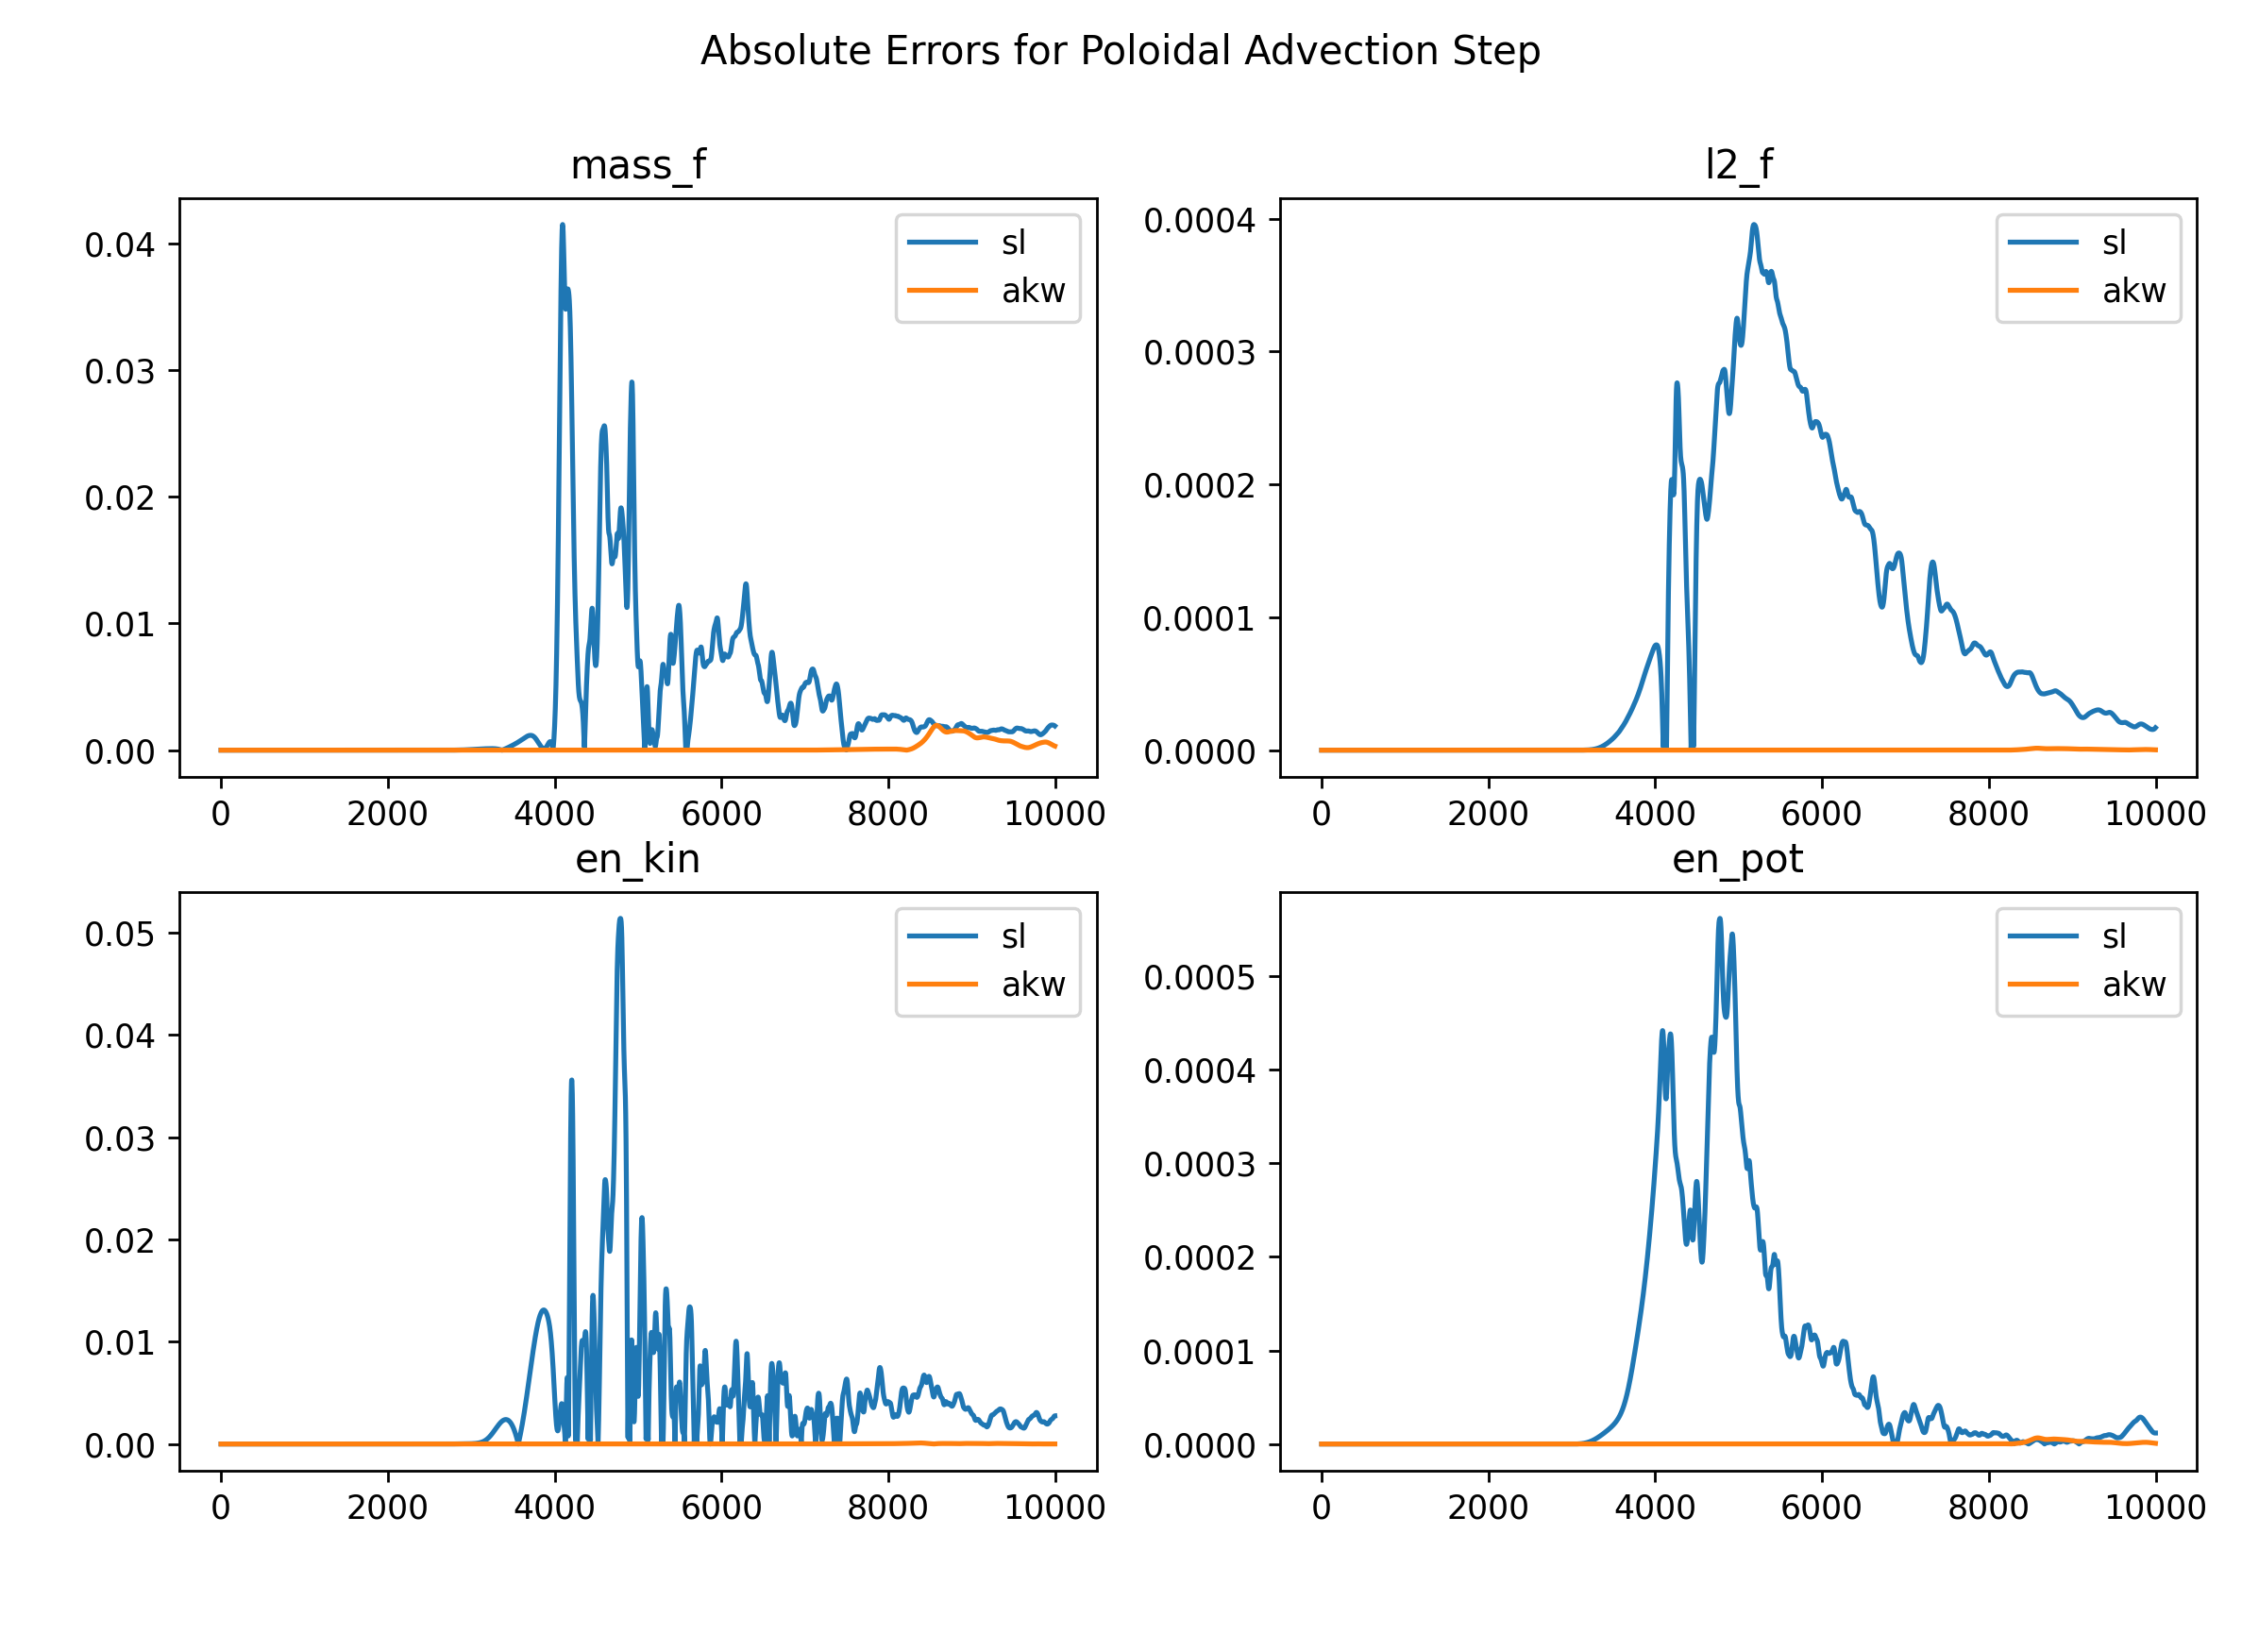
\includegraphics[width=0.9\linewidth]{plots/abs_err dt2}
	\caption{The absolute error for different quantities before and after the poloidal advection step with time step-size $\Delta t = 2$.}
	\label{fig:abserr_dt2}
\end{figure}


\begin{figure}
	\centering
	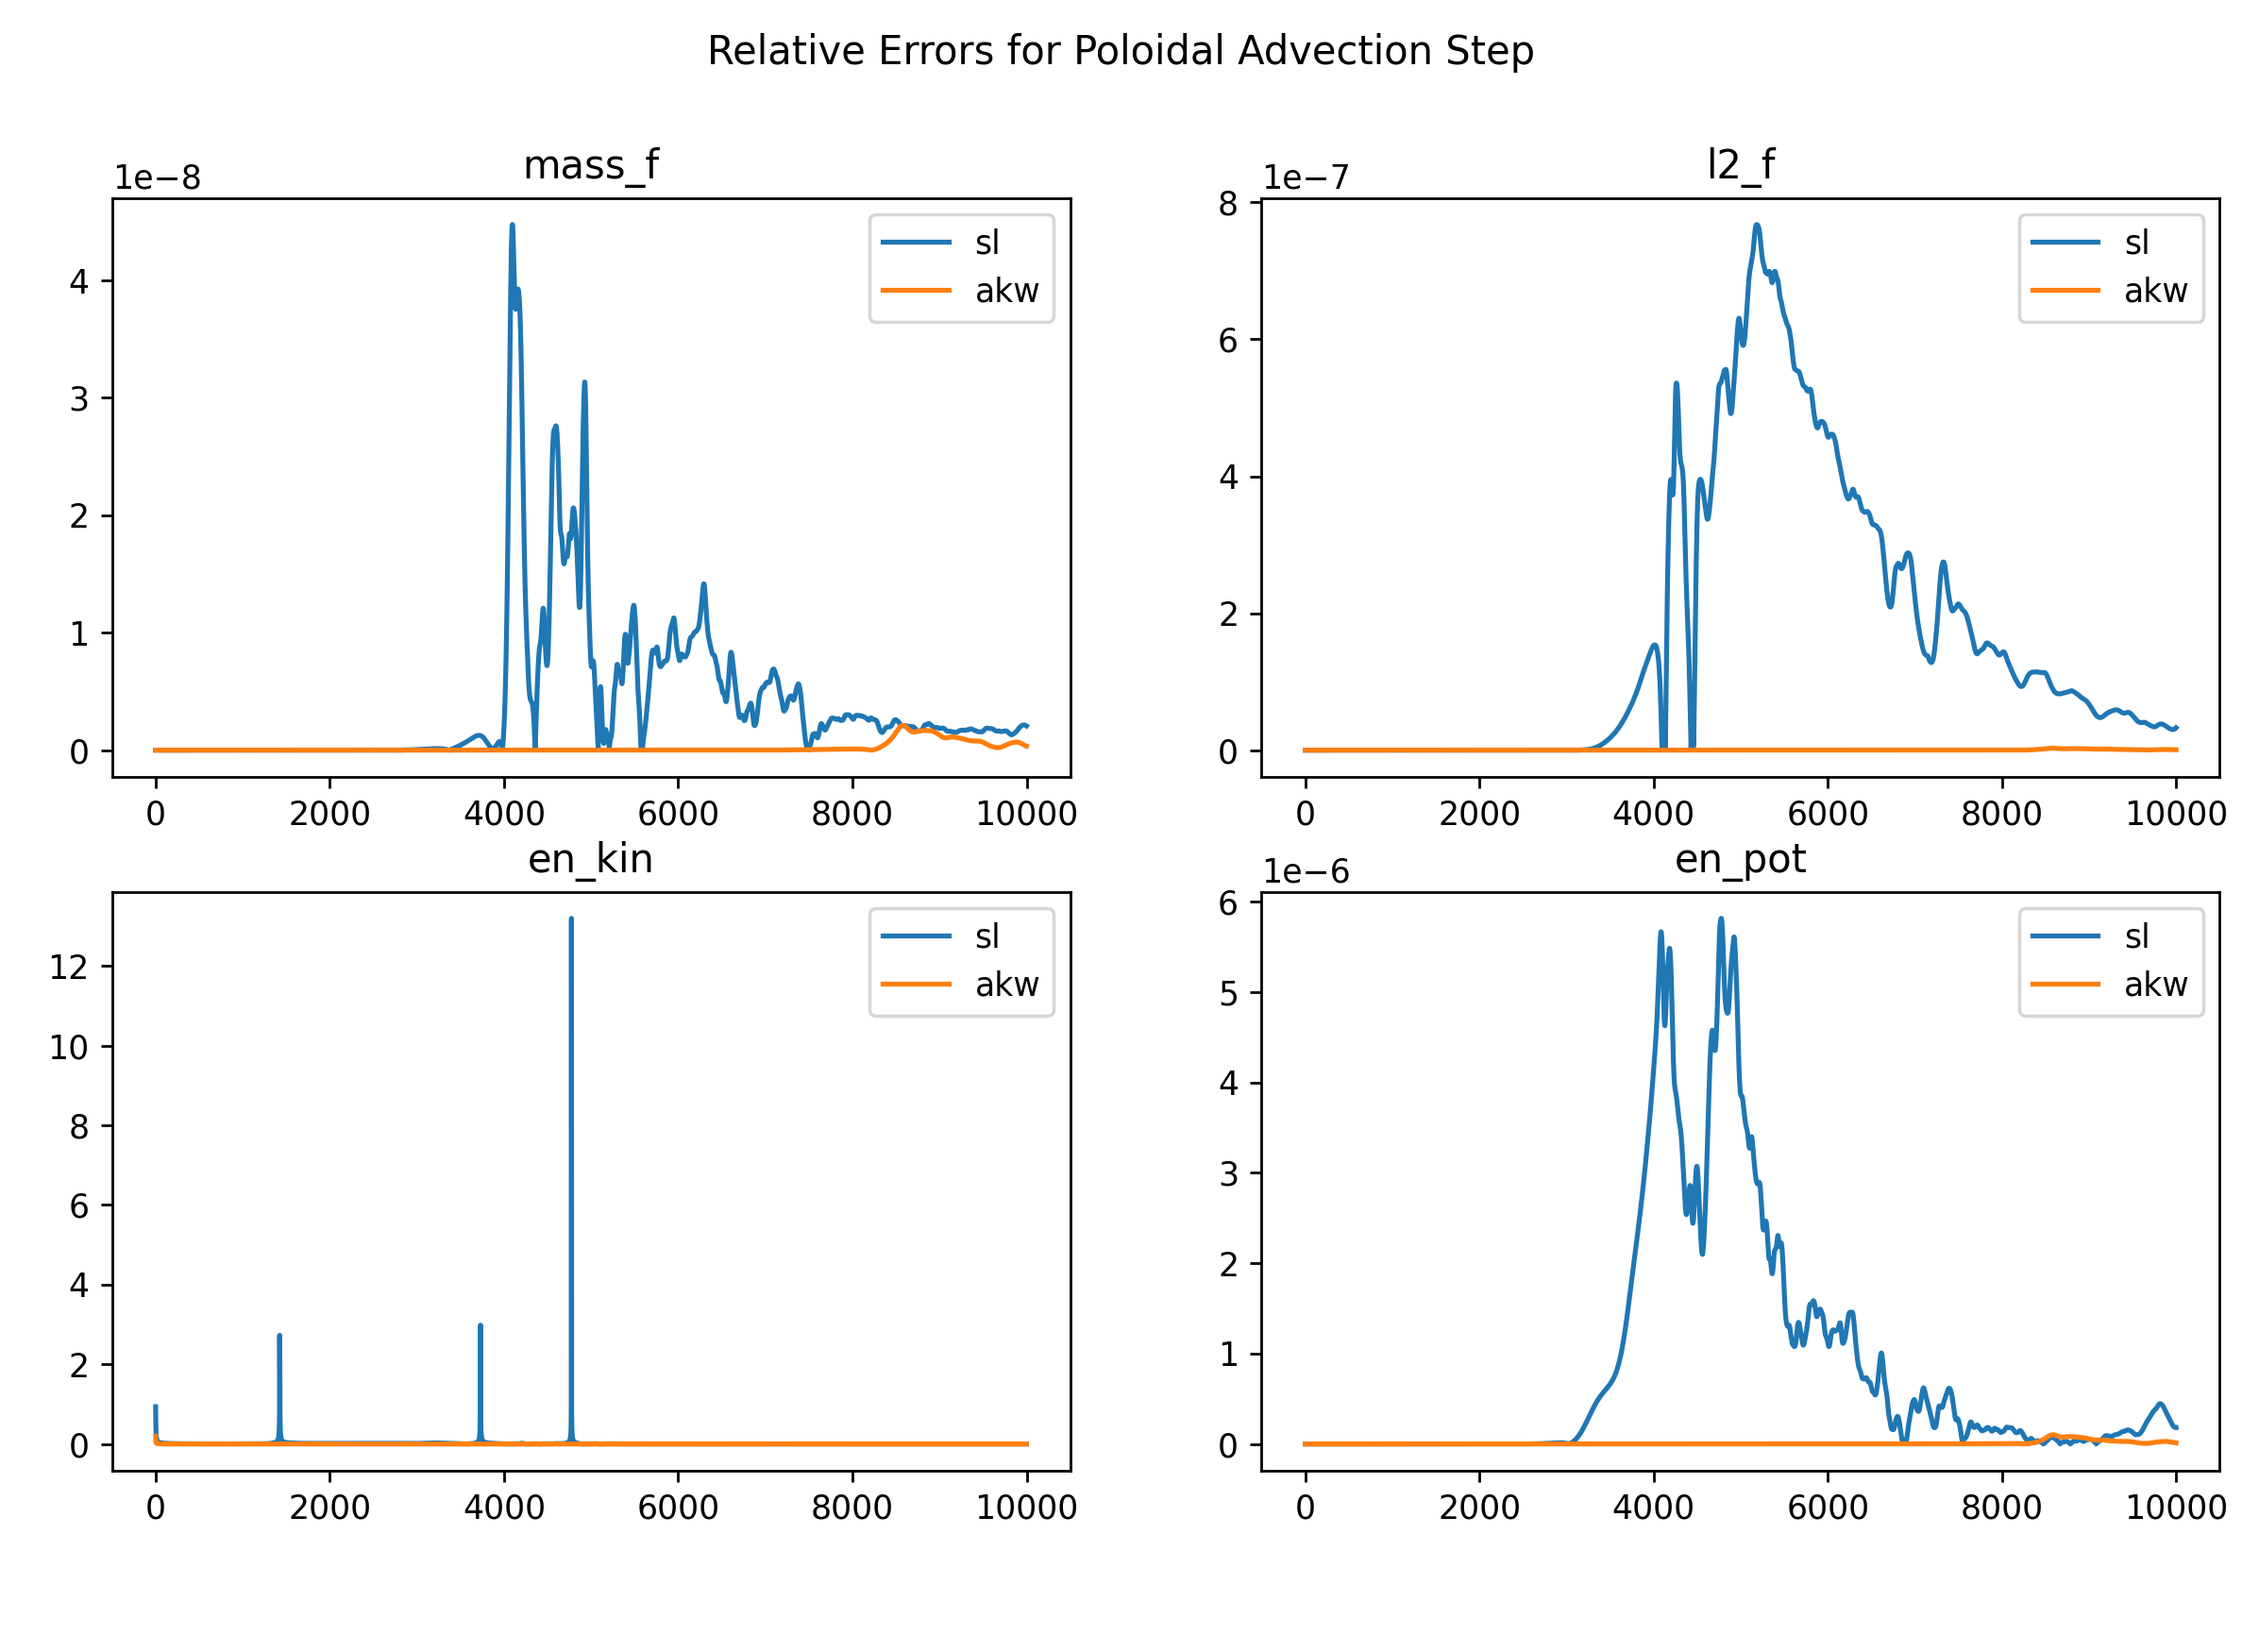
\includegraphics[width=0.9\linewidth]{plots/rel_err dt2}
	\caption{The relative error for different quantities before and after the poloidal advection step with time step-size $\Delta t = 2$.}
	\label{fig:relerr_dt2}
\end{figure}


\begin{figure}
	\centering
	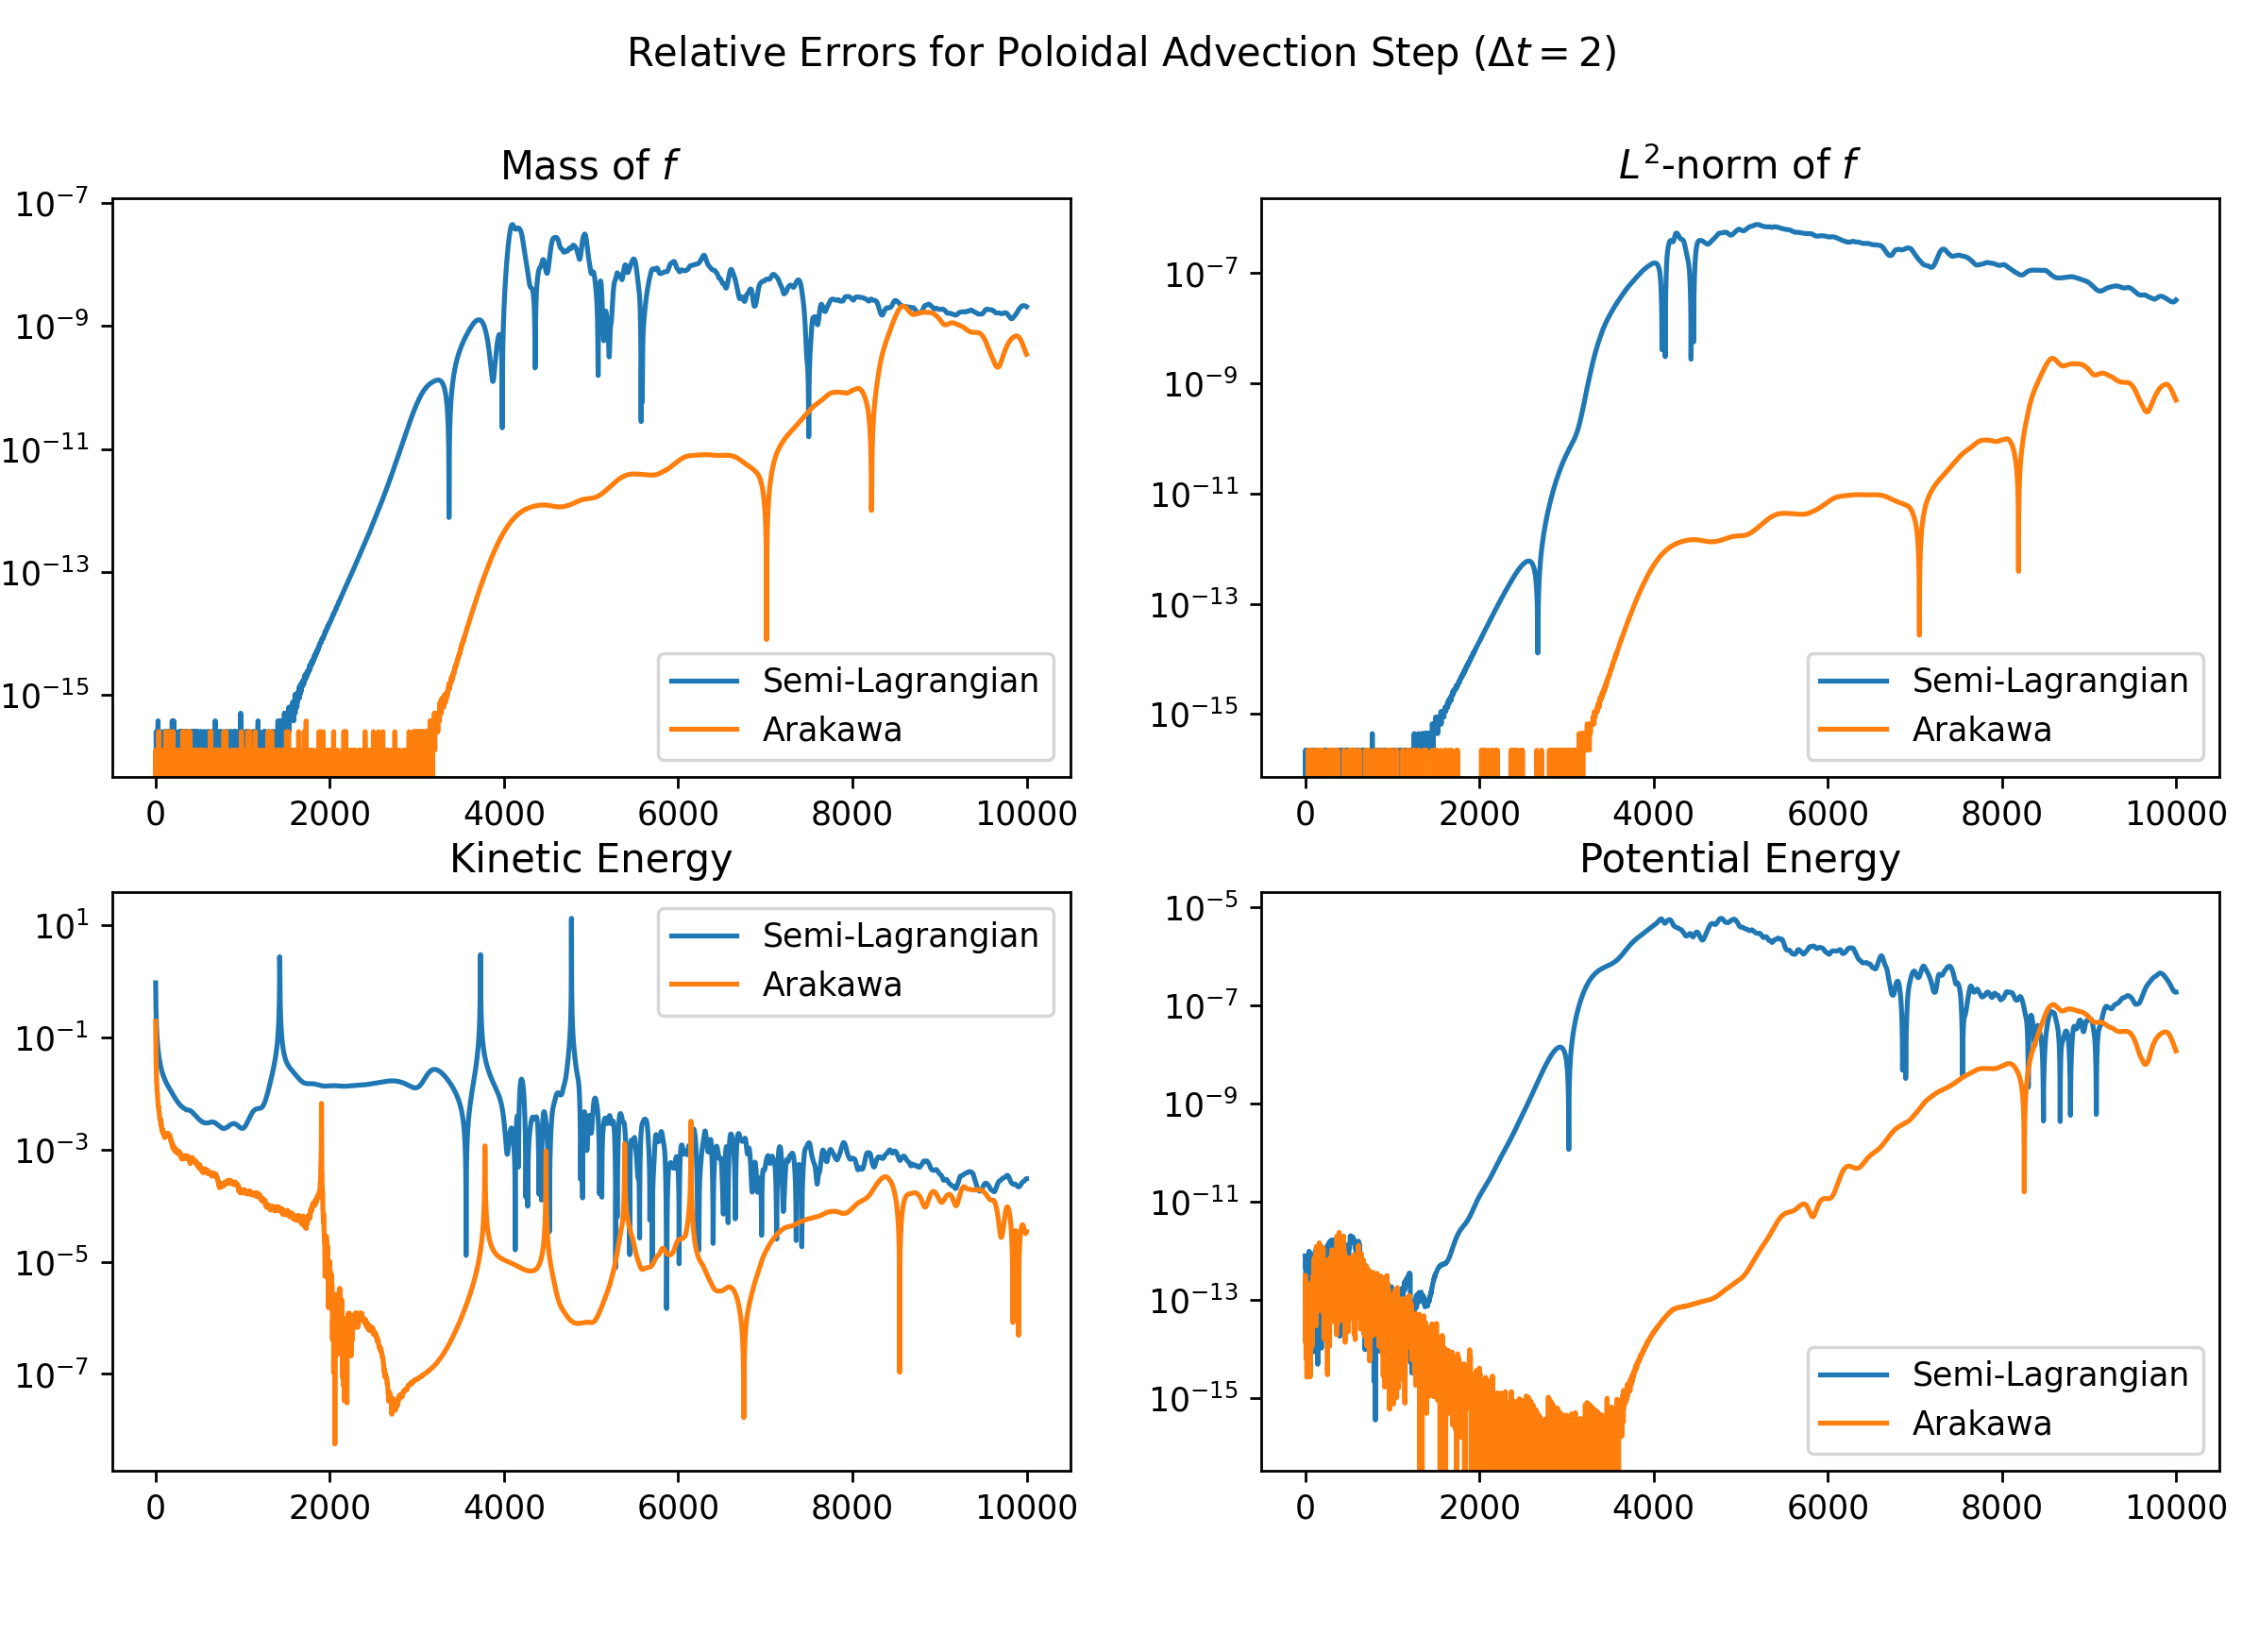
\includegraphics[width=0.9\linewidth]{plots/rel_err_log dt2}
	\caption{The relative error for different quantities before and after the poloidal advection step on a semi-logarithmic scale with time step-size $\Delta t = 2$.}
	\label{fig:relerrlog_dt2}
\end{figure}


\begin{figure}
	\centering
	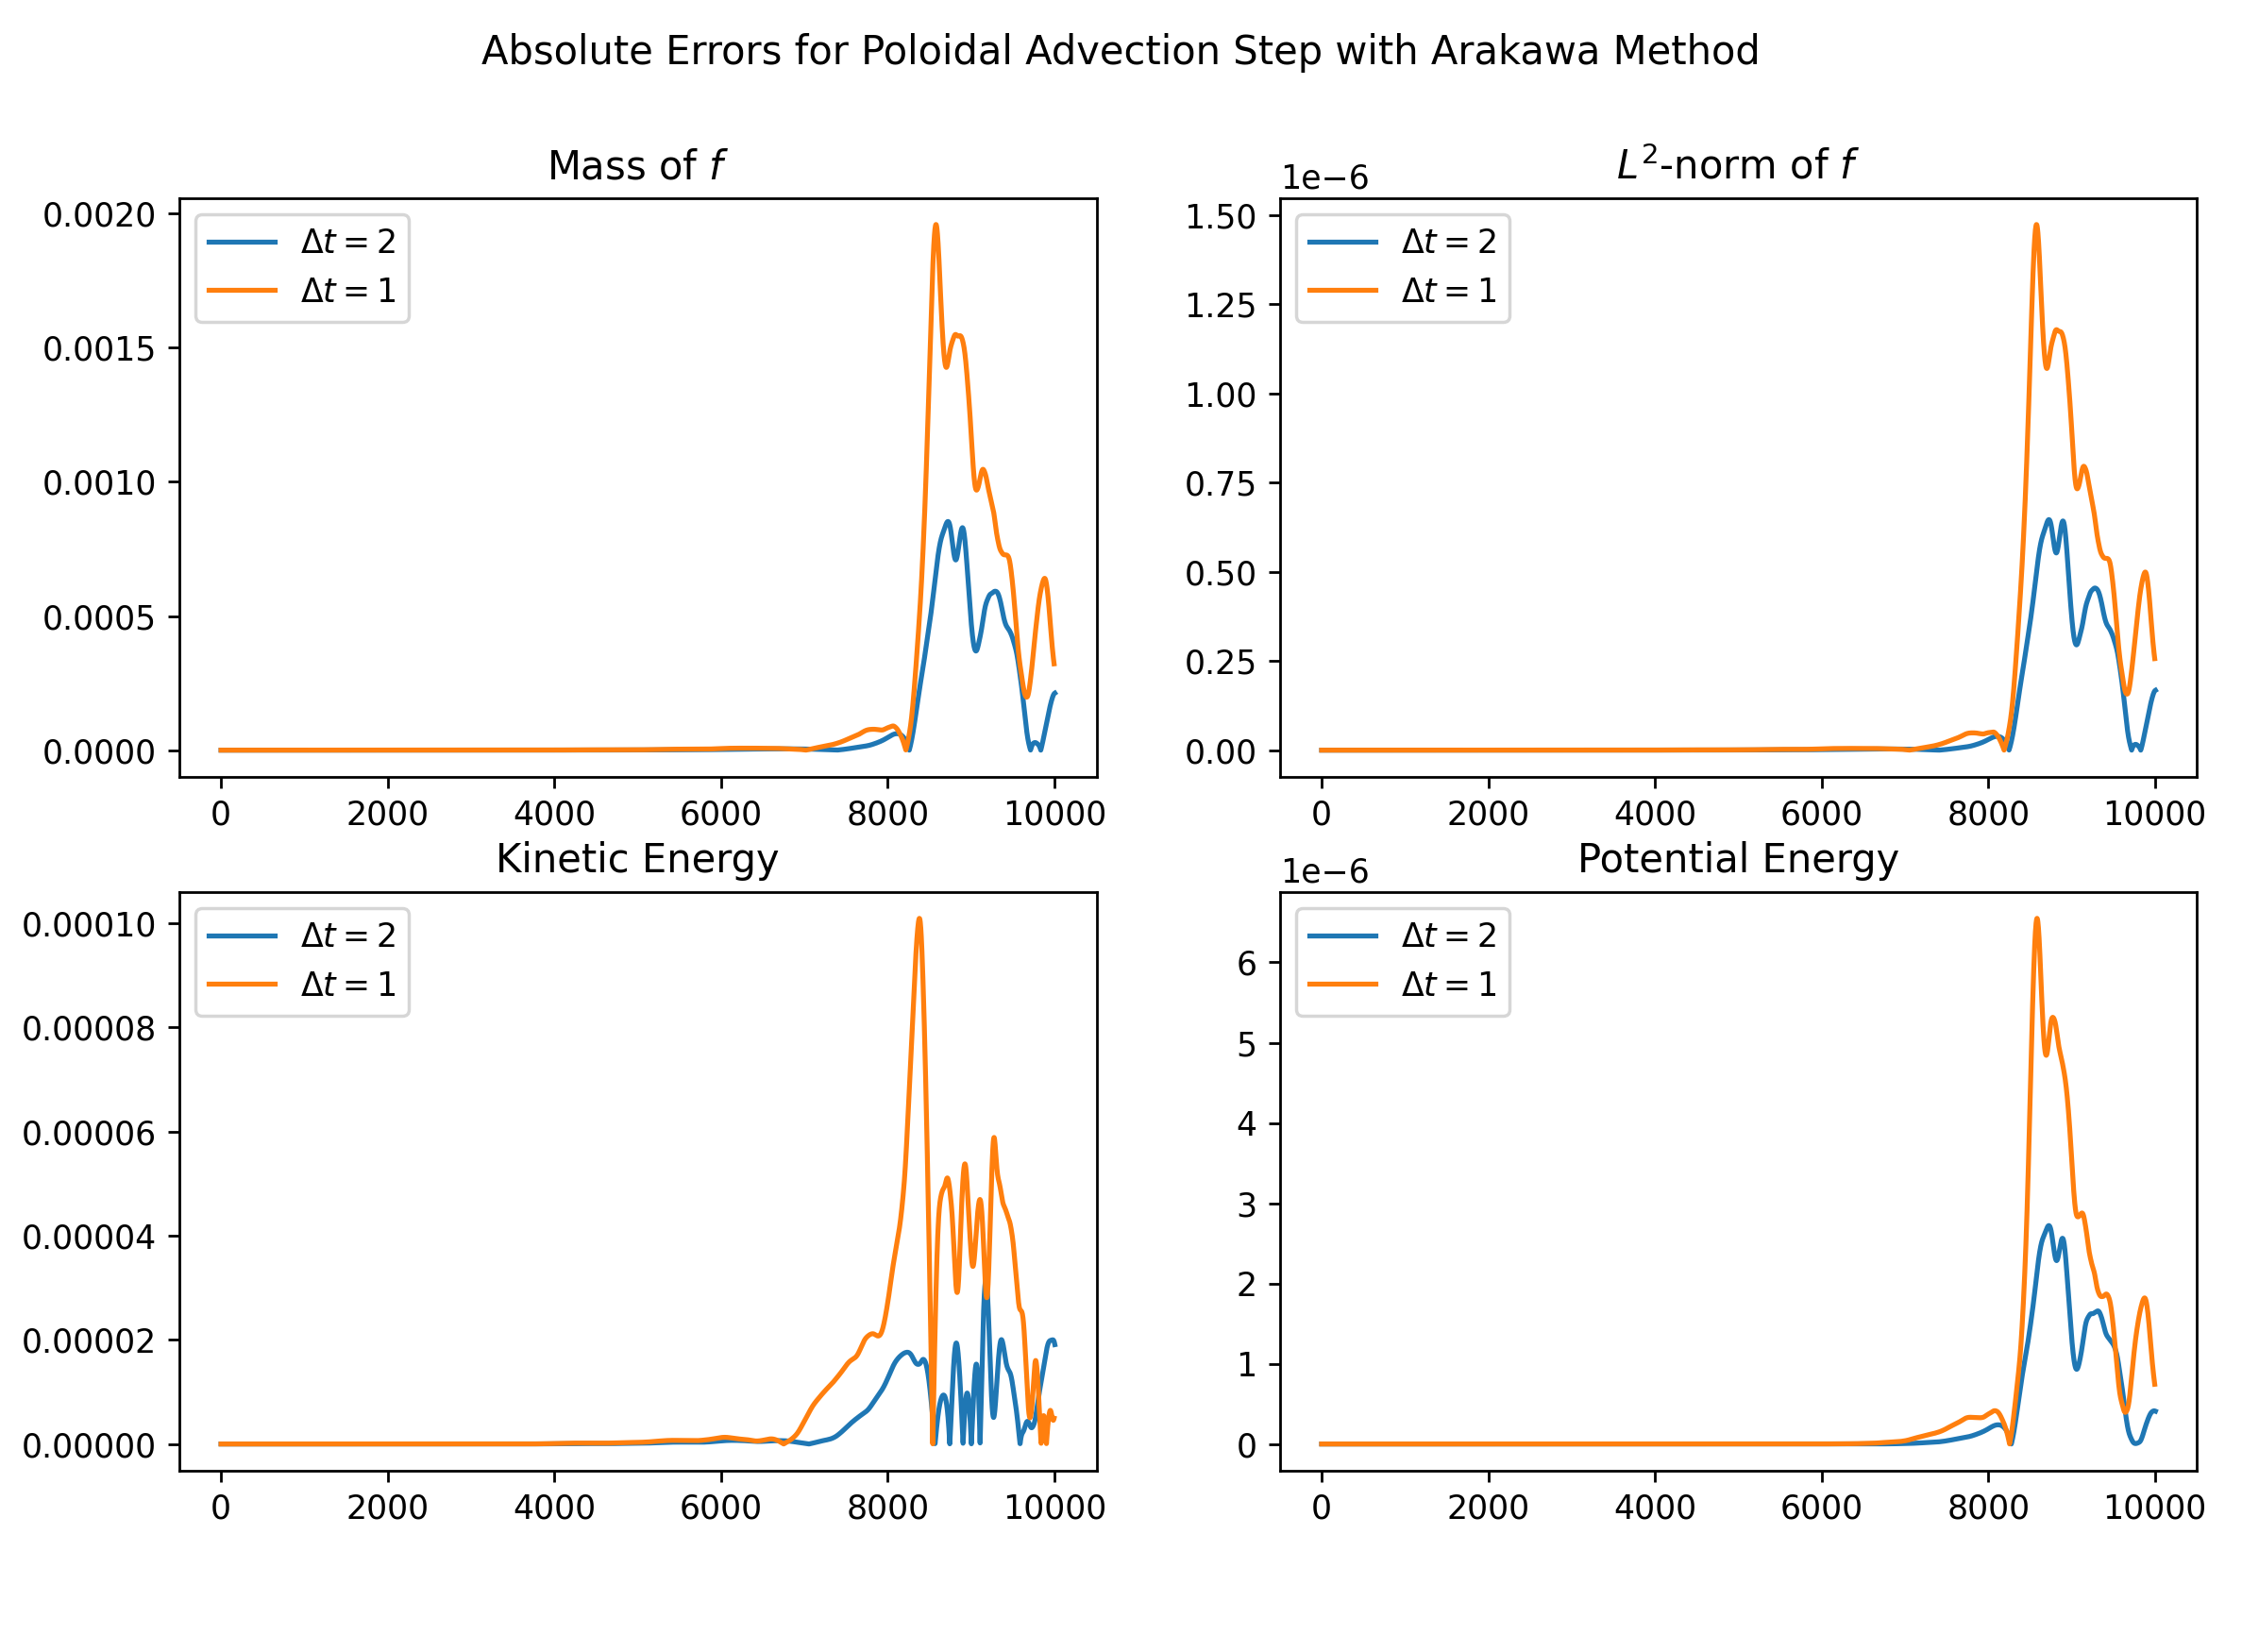
\includegraphics[width=0.9\linewidth]{plots/abs_err akw}
	\caption{The absolute error for different quantities before and after the poloidal advection step with the Arakawa method, comparing time step-size $\Delta t = 1$ and $\Delta t = 2$.}
	\label{fig:abserr_akw}
\end{figure}


\begin{figure}
	\centering
	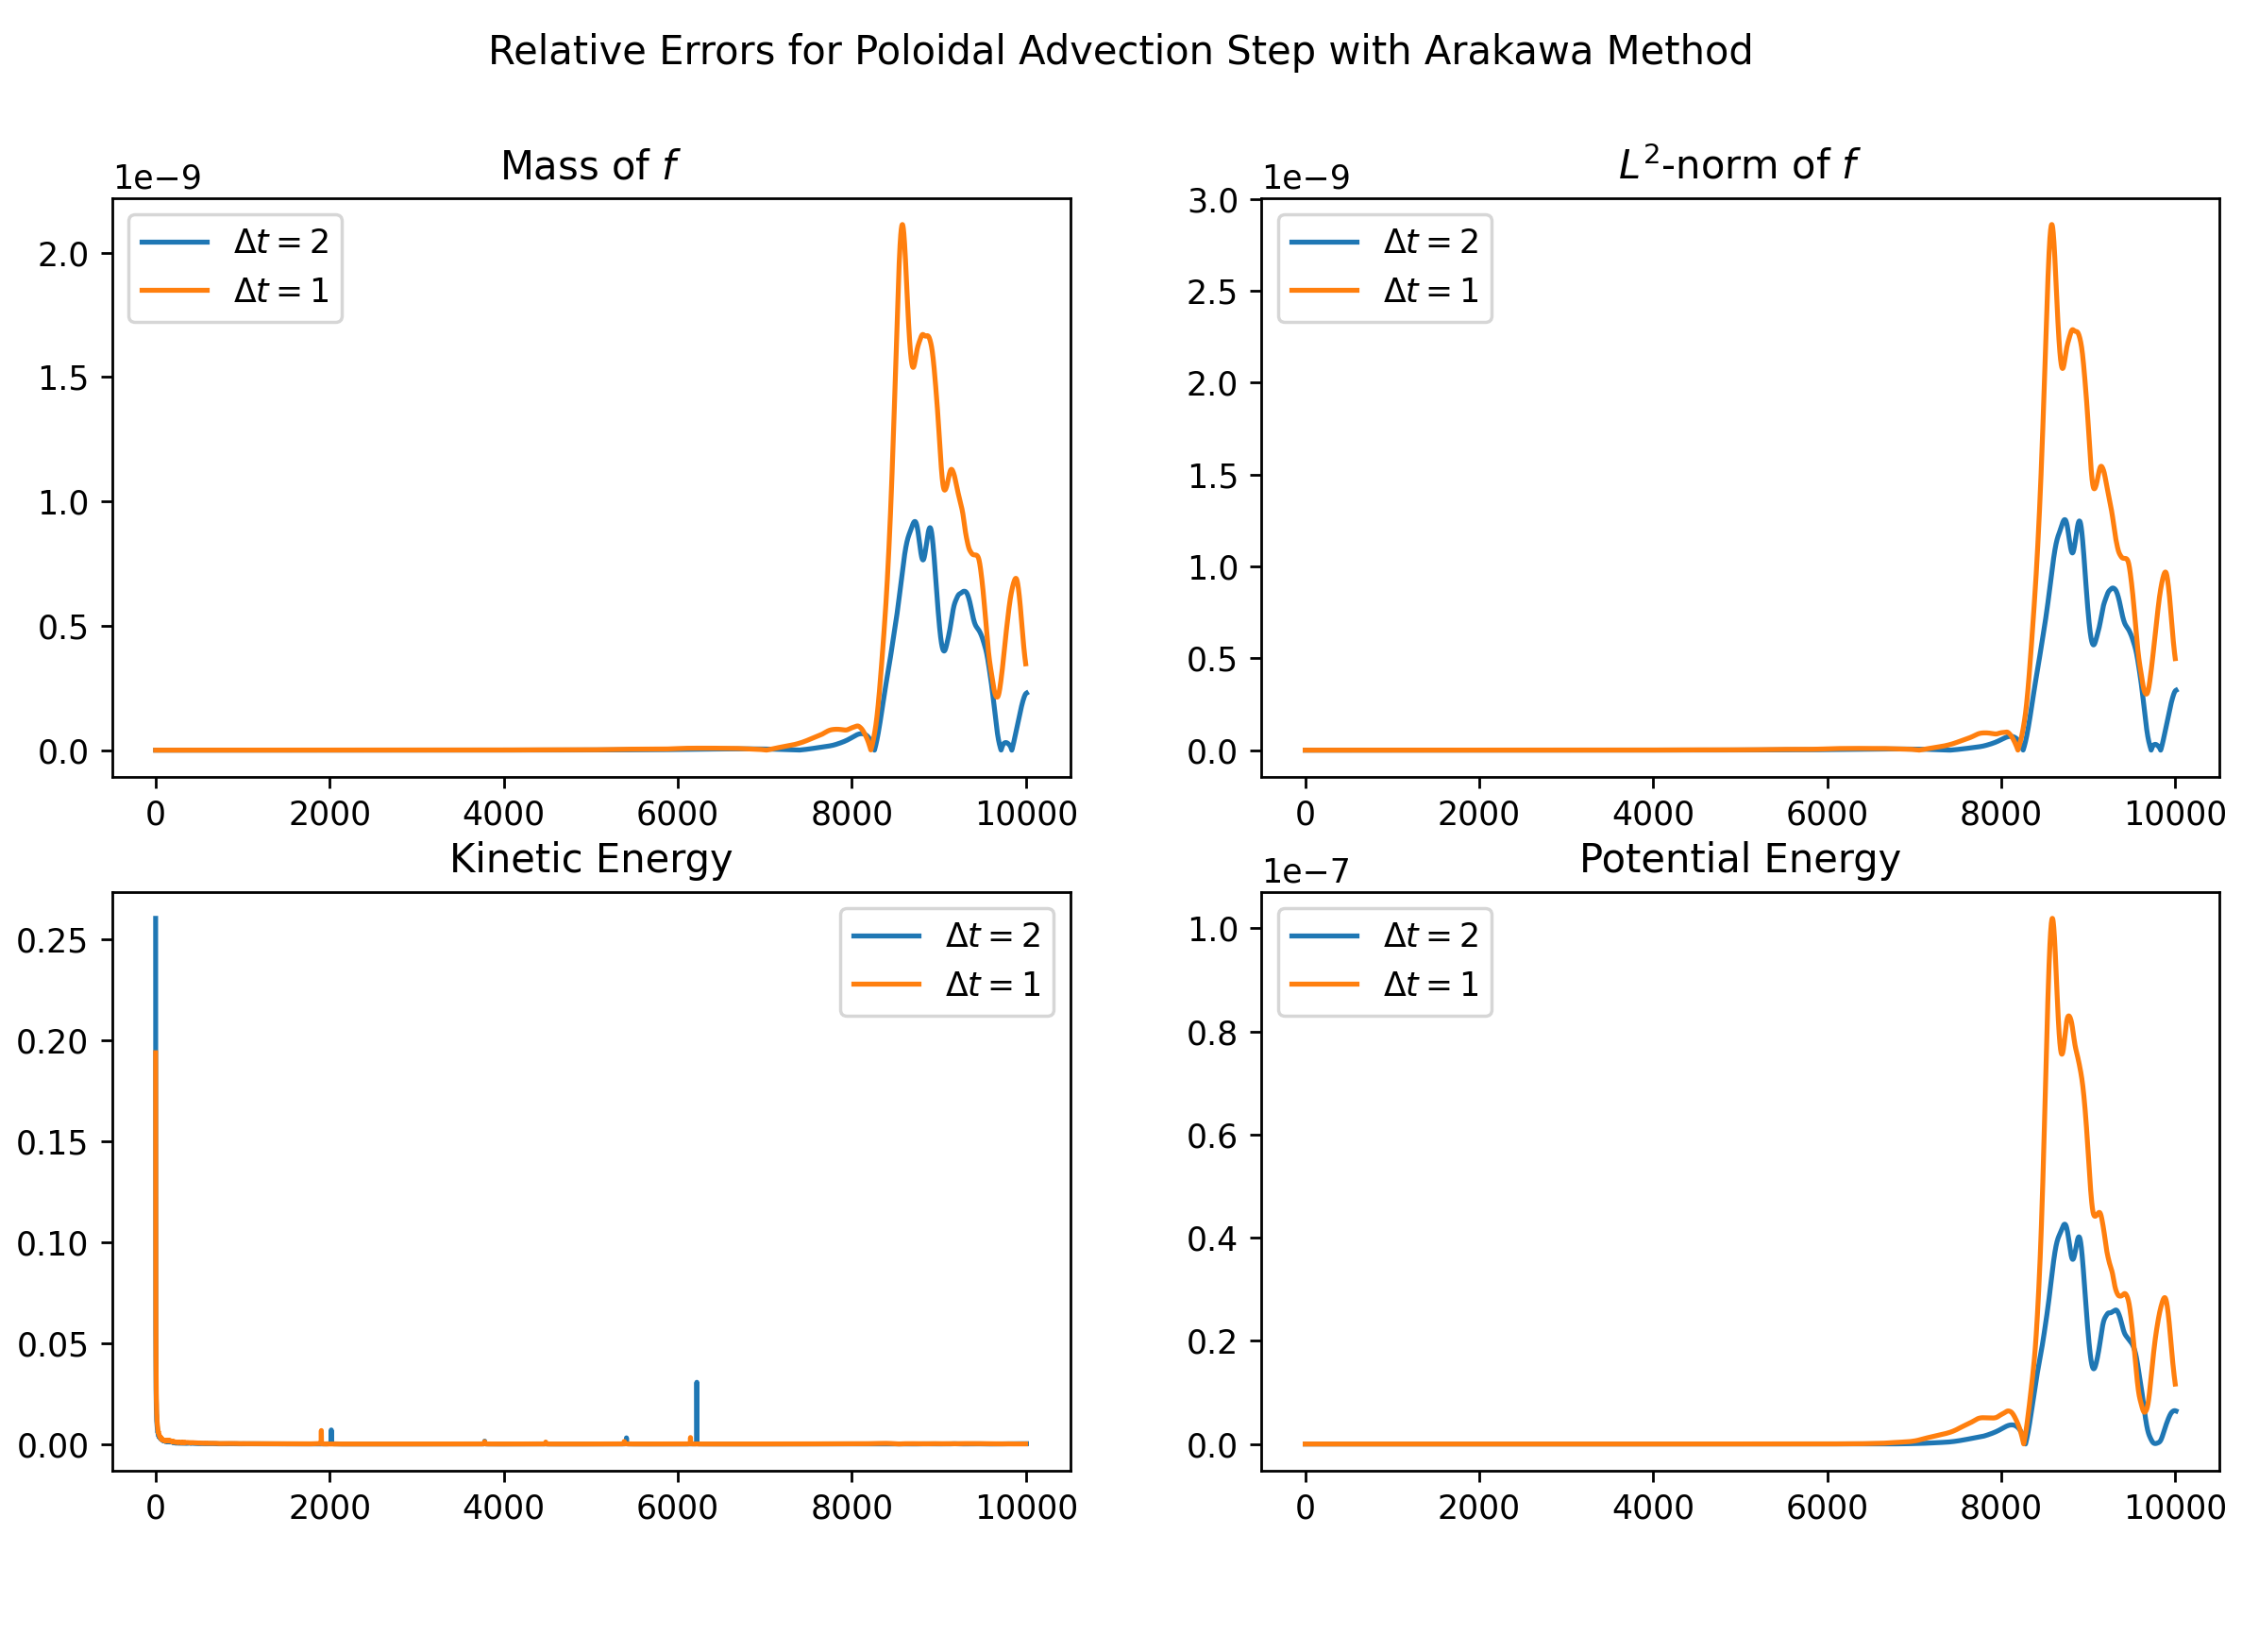
\includegraphics[width=0.9\linewidth]{plots/rel_err akw}
	\caption{The relative error for different quantities before and after the poloidal advection step with the Arakawa method, comparing time step-size $\Delta t = 1$ and $\Delta t = 2$..}
	\label{fig:relerr_akw}
\end{figure}


\begin{figure}
	\centering
	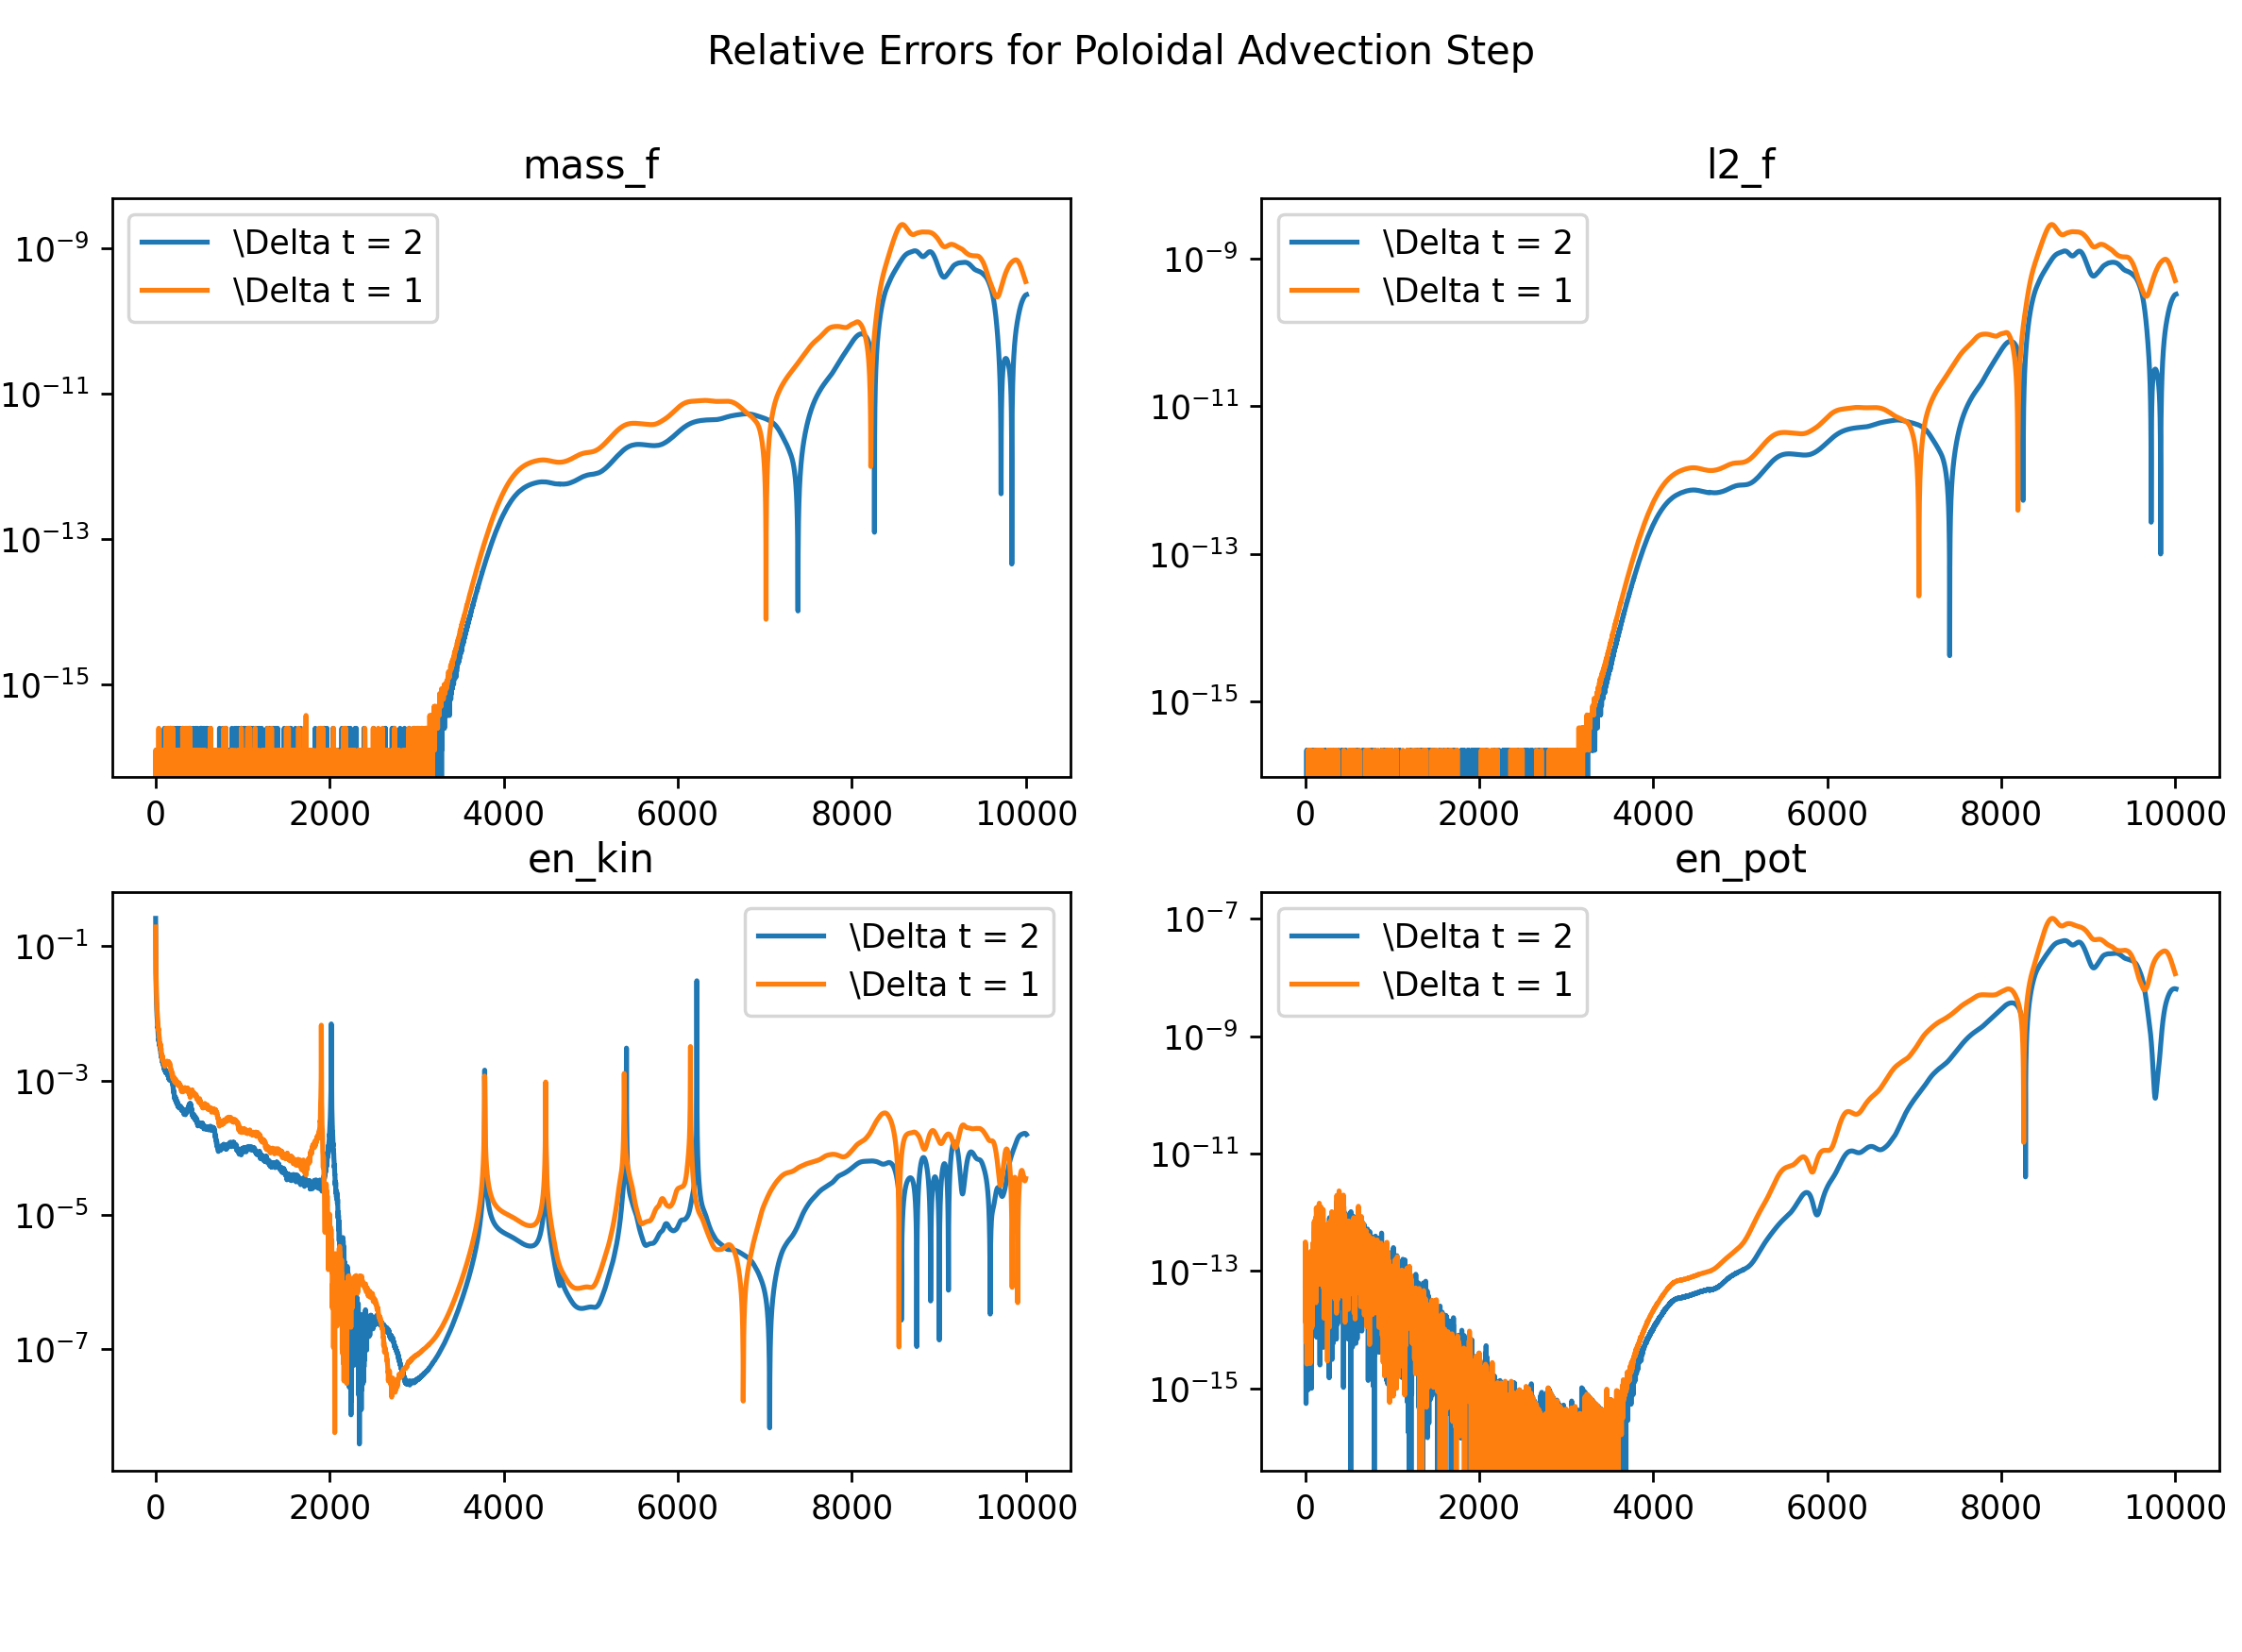
\includegraphics[width=0.9\linewidth]{plots/rel_err_log akw}
	\caption{The relative error for different quantities before and after the poloidal advection step on a semi-logarithmic scale with the Arakawa method, comparing time step-size $\Delta t = 1$ and $\Delta t = 2$..}
	\label{fig:relerrlog_akw}
\end{figure}



